\documentclass{article}

\usepackage{fancyhdr}
\usepackage{setspace}
\usepackage{titlesec}
\usepackage{tocloft}
\usepackage{lipsum}
\usepackage[fleqn]{amsmath}
\usepackage{amssymb}
\usepackage{hyperref}
\usepackage{url}
\usepackage{graphicx}
\usepackage{geometry}
\usepackage{enumitem}
\usepackage{parskip}
\usepackage{chemfig}
\usepackage{pdfpages}
\usepackage{tikz}
\usepackage{fancybox}
\usepackage{makecell}
\usepackage{pgfplots}
\usepackage{soul}
\usepackage{multirow}
\usepackage{ulem}
\usepackage{wrapfig}
\usepackage{subcaption}
\usepackage[T1]{fontenc}
\usepackage{esvect}
\usepackage{xcolor}
\usepackage{booktabs}
\usepackage{array}
\usepackage{colortbl}
\usepackage{fontspec}
\usepackage{tabularx}
\usepackage{pdflscape}
\usepackage{wasysym}
\usetikzlibrary{arrows}
\usetikzlibrary{decorations.pathreplacing}
\pgfplotsset{compat=1.17}
\definecolor{darkgreen}{RGB}{0, 160, 0}

\geometry{
    a4paper,
    total={170mm, 257mm},   
    left=20mm,
    top=20mm
}   

\hypersetup{
    colorlinks=true,
    linkcolor=black,
    urlcolor=blue,
    pdftitle={Team 31_Review 3 HS24}
}

\pagestyle{fancy}
\fancyhf{}
\fancyhead[L]{\leftmark}
\fancyhead[R]{\thepage}
\renewcommand{\headrulewidth}{0.4pt}

% === BIBLIOGRAPHY ===
\usepackage[utf8]{inputenc}
\usepackage{csquotes}
\usepackage[style=apa, backend=biber, doi=true, url=true]{biblatex}
\addbibresource{ref.bib}
\DeclareFieldFormat[article]{volume}{\textbf{#1}}
\DeclareFieldFormat[article]{journaltitle}{\textit{#1}}
% ====================

\newcommand{\figbox}[1]{ 
    \begin{figure*}[ht!]        
        \begin{center}            
            \fbox{#1}        
        \end{center}    
    \end{figure*}
}

\newcommand{\wrapfill}{
    \par
    \ifnum \value{WF@wrappedlines} > 0
        \addtocounter{WF@wrappedlines}{-1}%
        \null\vspace{
            \arabic{WF@wrappedlines}
            \baselineskip
        }
        \WFclear
    \fi
    \phantom{}
}

\newcommand{\difference}{\,\backslash\,}
\newcommand{\rem}{\underline{Remark}: }
\newcommand{\nots}{\underline{Notation}: }
\newcommand{\prf}{\underline{Proof}: }
\newcommand{\exs}{\underline{Example}: }
\newcommand{\defs}{\underline{Definition}: }
\newcommand{\wrn}{\underline{Warning}: }
\newcommand{\sht}{\ |\ }
\newcommand{\pph}[1]{\paragraph{#1} \phantom{}\\}
\newcommand{\dm}{\displaystyle}
\newcommand{\rad}{^{\mathrm{c}}}
\newcommand{\myc}{My$_{\text{celium}}$Tent}

\titleformat{\chapter}[block]{\bfseries\Large}{\thechapter.}{1em}{}

\definecolor{newgreen}{HTML}{4da833}
\definecolor{neworange}{HTML}{e96d2f}
\definecolor{newblue}{HTML}{145d80}

%========= TEXT ===========

\begin{document}

\hypersetup{citecolor=black}

\begin{titlepage}
    \begin{wrapfigure}{l}{7.5cm}
        \hspace*{.01cm}
        
\includegraphics[width=.3\textwidth]{media/hslu-logo-2.png}

        \vspace*{.01cm}
        \hspace*{.16cm}
\includegraphics[width=0.4\textwidth]{media/hslu-svg-logo.png}
    \end{wrapfigure}

    \phantom{}
    \vspace*{-1cm}

    \begin{flushright}
        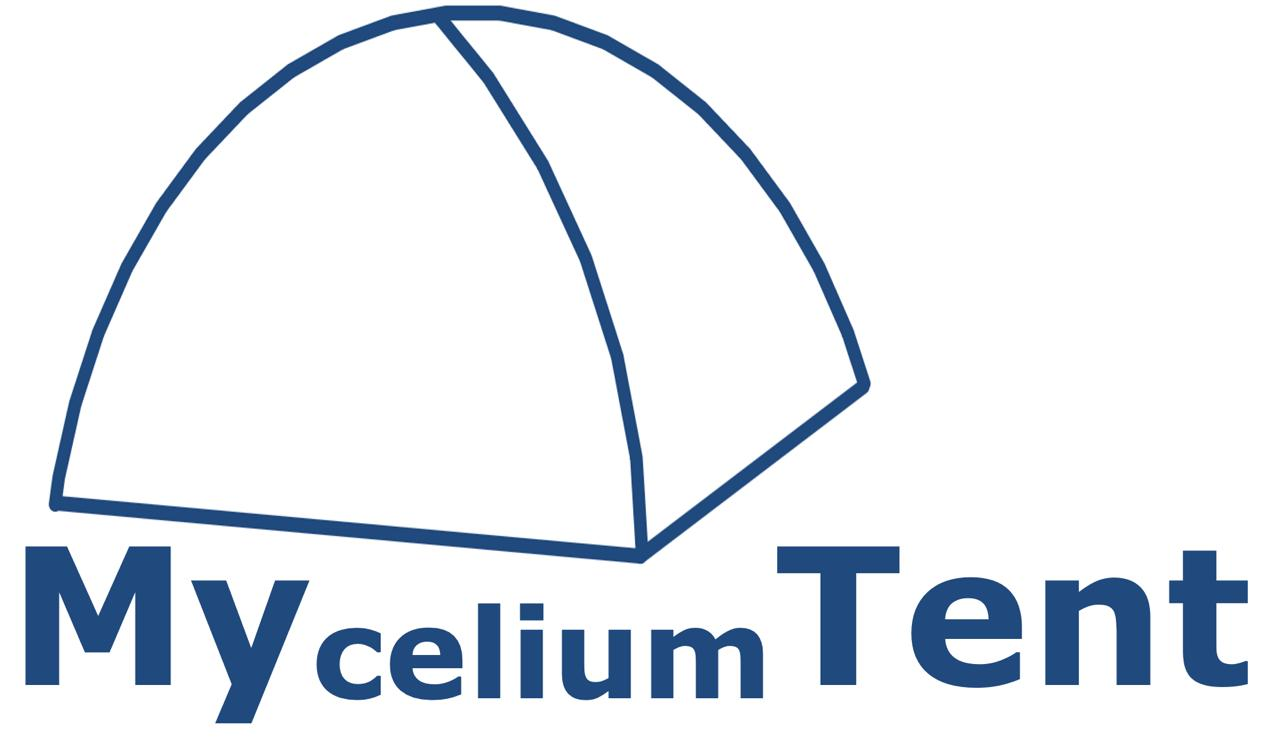
\includegraphics[width=.3\textwidth]{media/mytent_logo.jpeg}
    \end{flushright}

    \wrapfill

    \vspace*{-3.5cm}
    {\huge \textbf{Project Context 1}}

    {\Large Final Report}

    \vspace*{3cm}
    \begin{center}
        {\Huge \textbf{My$_{\text{celium}}$Tent}}

        \vspace*{.1cm}
        \textbf{\large The biodegradable tent}
    \end{center}

    \vfill
    {\Large \textbf{Team 31}}\\
    {\large \vspace*{.01cm}
        Althaus Simon\\
        \vspace*{.01cm}
        Berner Nic\\
        \vspace*{.01cm}   
        Frongillo Matteo\\
        \vspace*{.01cm}
        McCarthy Benjamin\\
        \vspace*{.01cm}
        Nyamdorj Narandavaa\\
        \vspace*{.01cm}
    }
    
    \vspace{1cm}
    {\large Horw, 18th December 2024}
\end{titlepage}

\newpage
\section*{Team 31}
\renewcommand{\arraystretch}{1.5}
\begin{tabular}{@{}p{0.21\textwidth}p{0.42\textwidth}p{0.3\textwidth}@{}}
\textbf{Name} & \textbf{Field of studies} & \textbf{E-mail} \\
Althaus Simon & Business engineering & \href{mailto:simon.althaus@stud.hslu.ch}{simon.althaus@stud.hslu.ch} \\
Berner Nic & Energy and environmental systems engineering & \href{mailto:nic.berner@stud.hslu.ch}{nic.berner@stud.hslu.ch} \\
Frongillo Matteo & Energy and environmental systems engineering & \href{mailto:matteo.frongillo@stud.hslu.ch}{matteo.frongillo@stud.hslu.ch} \\
McCarthy Benjamin & Medical engineering | Life sciences & \href{mailto:benjamin.mccarthy@stud.hslu.ch}{benjamin.mccarthy@stud.hslu.ch} \\
Nyamdorj Narandavaa & Business engineering & \href{mailto:narandavaa.nyamdorj@stud.hslu.ch}{narandavaa.nyamdorj@stud.hslu.ch} \\
\end{tabular}

\section*{Declaration of academic integrity}
\noindent\fbox{%
    \parbox{\textwidth}{%
        \vspace{0.3cm}
        {\itshape
        The authors confirm with their signature that this piece of work was written independently, without support from third parties and without the use of tools other than those specified.
        
        \vspace{0.5cm}
        Where we have taken advantage of the work and ideas of others (including electronic sources), we have given full acknowledgement.
        
        \vspace{0.5cm}
        This piece of work has not been presented in the same or similar form.
        }

        \vspace{0.8cm}
        \begin{tabular}{@{}p{0.5\textwidth} p{0.5\textwidth}@{}}
        \textbf{Date / Location:} \newline \newline 11th December 2024, Horw & 
        \textbf{Signatures:} \newline 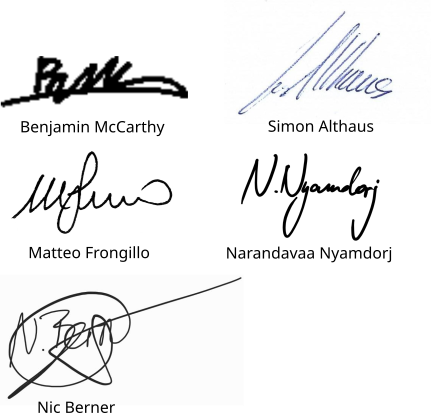
\includegraphics[width=0.45\textwidth]{media/signatures.png} \\
        \end{tabular}
        
        \vspace{0.5cm}
    }%
}

\newpage
\section*{Abstract}
Festivals are significant cultural events but contribute to
substantial environmental challenges, particularly through waste
generated by abandoned, low-cost tents often damaged and left behind.
These tents are usually composed of synthetic materials that are
difficult to recycle or dispose of responsibly, exacerbating
ecological issues. 

This study explores the potential for designing a festival tent that
meets user requirements while addressing the environmental impact of
single-use camping gear.  

Through a value-benefit analysis, mycelium was identified as an
optimal material due to its biodegradability, recyclability, and
structural viability. The proposed design, the \myc,
aligns with circular economic principles, offering a fully recyclable
and predominantly biodegradable alternative to traditional festival
tents. 

Although experimental validation under simulated outdoor conditions
has not yet been conducted, the material is expected to exhibit
adequate water resistance and structural integrity for short-term use.
Future testing is required to confirm these properties and refine the
material for broader applications. 

The \myc\ represents a sustainable, cost-effective solution to
reduce festival waste and promote environmentally responsible
practices. It emphasizes the potential of mycelium-based materials in
advancing renewable and circular design solutions, underscoring the
need for further research and development in this field.

\newpage
\tableofcontents
\thispagestyle{empty}

\newpage
\section{Introduction}
The environmental challenges posed by global warming have driven society to adopt
increasingly eco-friendly practices. However, certain events, such as music festivals,
still leave a considerable environmental footprint. Festivals worldwide produce vast
amounts of waste, reaching up to 100 tons per day, with abandoned nylon tents being one
of the most persistent issue \parencite{Gray2019}. These tents, often made
from synthetic materials, are not easily recycled or biodegradable, contributing
significantly to plastic pollution that could otherwise be mitigated.

This report focuses on addressing this issue by introducing an innovative solution: a
fully biodegradable and mostly recyclable tent made of mycelium. Mycelium, derived from
fungal root structures, provides an environmentally friendly alternative to traditional
materials, aligning with circular economy principles \parencite{attias}. This project
aims to design a tent that meets user needs while reducing waste and improving disposal
options at the end of its life cycle.

This report presents the project in its developmental stages. Section 2 explores the
properties and potential of mycelium for the described application. Section 3 outlines the
requirements and methodologies, including a morphological box and a value-benefit
analysis, used to determine the final design. The resulting product concept is detailed in
Section 4, followed by its validation and testing, discussed in Section 5. Lastly,
Section 6 concludes by evaluating the success of the project and identifying opportunities
for future improvements.


\newpage
\section{Background}
This section provides the essential background for the project, focusing on mycelium as a
sustainable material for tent construction. It examines its properties, potential
applications, and environmental benefits, alongside an analysis of tent structures, market
trends, and safety requirements. This foundation supports the development of the \myc\ as
an eco-friendly and functional solution.

\subsection{Mycelium}
The development of the MyceliumTent is focused on replacing existing nylon and plastic
tent fabrics with a mycelium-based fabric in order to make it recyclable.

\subsubsection{Definition}
Mycelium is the underground root network created by a mushroom organism. Fungi
nourish themselves by secreting digestive enzymes to break down organic material in
their surroundings and absorb it through the cell walls of the hyphae, their root network
\parencite{fungus}. Various types of fungi produce mycelium. For this project, the focus
is on a fungus with a high growth rate, suitable for the production of biocomposites. In
this case, it is possible to use the oyster mushroom \parencite{mushroom}.

\subsubsection{Potential of mycelium}
The potential of this material lies in its low carbon footprint, low energy and processing
cost, and biodegradability. The most common use
cases in the industry so far include leather, packaging materials, or composites used for
construction. However, challenges remain, such as the lack of standardized treatment
methods during material development. This project specifically explores
biodegradability, durability, water, and fire resistance, as needed to construct a tent
fabric \parencite{ALANEME2023234}.

\subsubsection{Mylo leather}
Mylo is a product made by the company Bolt Threads, designed as an alternative to animal
leather. It is made of a foam-like mycelium \parencite{myloleather} and
is both sustainable and biodegradable. Its durability, waterproofness, and lightweight
nature make it a promising material for applications such as tent construction, aligning
with eco-friendly design principles.

\subsection{Environment}
This chapter explores different properties of mycelium bio-composites (MBC), which is the
material used in this project. MBCs are ``composed of an agricultural residue, a non-living
material, colonized by a fungus'' \parencite{amziane2023bio, p. 740}. As of today, the full
potential of MBCs has not been found, and different production processes and growth
combinations, i.e. types of fungi and substrates continue to be tested and compared.

\subsubsection{Mycelium bio-composites}
Some important properties for this product are sound absorption, thermal conductivity, and
moisture buffering value. These properties vary greatly depending on the substrate-fungus
combination. Research on fifty unprocessed MBCs found that the sound absorption coefficient
differs from 0.5 to 0.95 depending on the frequency, indicating they are good sound
absorbers (\cite{amziane2023bio, p.749}). The thermal conductivity value was found to be
between 0.057 -- 0.085 W/(mK), and the mean moisture buffering value was 1.632
(\cite{amziane2023bio, p.749}). However, no clear values of water resistance were found,
although it is possible to coat the MBC in biodegradable polyurethanes or beeswax for
extra water resistance and smoothness \parencite{amziane2023bio}.

\subsubsection{Mycelium-base leather}
One of the MBC products in use today is mycelium-based leather (MBL). Research has shown
that the order of polyporales fungi, specifically Fomitella fraxinea, in combination with
a substrate made of sawdust and rice bran, is best suited for the production of MBL. After
harvesting, the composites are plasticized (with a biodegradable mixture) and hot-pressed,
forming a leather-like material. These processes increase tensile strength, elongation
percentage, and reduce water absorption. MBL has a mean tensile strength of 8.49 MPa, can
elongate up to 58.86\%, and has a water contact angle of up to 129.63$^\circ$, making it
hydrophobic \parencite{jof8030317}. Considering these aspects, MBL has the highest
potential, of the current known MBC products, to be used for this project. 

\subsubsection{Biodegradability}
Depending on the fungi and substrate used, the biodegradation duration can vary.
For example, using Pleurotus ostreatus on a bamboo-based substrate coated with beeswax
for increased water resistance shows a mass reduction of 64.13\% after two months. However,
due to insufficient research on the biodegradability of other MBCs, no definitive
information can be provided on the biodegradability of class-sharing fungi like
polyporales \parencite{gan}. 

\subsection{Structure and setup}
There are several construction options available for tents. To determine the most suitable
option for the purposes of this study, this section evaluates the advantages and
disadvantages of the most common tent designs. Hilleberg, a manufacturer of high-quality
expedition tents, prioritises ease of use, which aligns with the criteria important for
the product. Therefore, their approach to tent construction serves as a relevant reference
for this analysis. Hilleberg categorizes its tents by label, with the Yellow Label being
the most applicable to this project's needs, as these tents are designed for use during
snow-free months and in protected environments, or in warmer climates \parencite{hilleberg2024b}.

The two most common constructions are Tunnel Tents and Dome Tents. Tunnel tents
provide the best space-to-weight ratio, making them ideal for mobile journeys where the
tent is frequently set up and taken down. Their lighter overall design is advantageous for
users who carry their gear during the day. However, tunnel tents are less stable in windy
or snowy conditions and typically require pegging to remain upright.

In contrast, dome tents offer greater stability, particularly in adverse weather conditions
such as snow or high winds. They are better suited for base camp setups, where they can
remain stationary for extended periods. Some dome tents are freestanding, which
eliminates the need for pegging and makes them useful in terrains like rocky or gravelly
soil. Despite these advantages, dome tents tend to be heavier and provide less space for
the weight they add \parencite{hilleberg2024a}. 

In addition to tunnel and dome tents, instant tents represent another construction option
that has gained popularity in recent years due to improvements in ease of setup. These
tents combine features of both tunnel and dome designs, offering a balance between
spaciousness and stability. Instant tents are particularly advantageous for users seeking
quick and simple setup, often requiring minimal effort. However, they are generally not
designed to withstand harsh environmental conditions such as strong winds or heavy
snow, making them more suitable for mild weather and less extreme environments
\parencite{outdoorlife2024}.

\subsection{Marketing}
The analysis of the marketing of camping tents and outdoor equipment is based on the use
of strategies leveraged to reach and engage consumers globally, in Europe, and Switzerland.
Nowadays, the use of social media is a key focus for product promotion and customer
loyalty through targeted advertising and influencers.

\subsubsection{Worldwide market}
In 2022, the global camping tent market reached a total value of USD 2.65 billion.
The future of this market is positive; in fact, it is set to grow further to USD 4 billion
by 2028. This positive outlook is possible due to the increase in outdoor recreation and
nature tourism \parencite{expertmarket2023}.

\subsubsection{European market}
According to reported projections, by 2029 the European camping tent market will grow
significantly, reaching a value of USD 1.50 billion. The analysis covers various product
categories, materials, and capacities, highlighting the increasing demand for innovative
and practical solutions in line with new camping trends \parencite{arizton2024}.

\subsubsection{Swiss market}
The analysis of the camping tent market in Switzerland focuses on growth trends driven by
increased outdoor activities and investment in sustainable materials. Changes in consumer
preferences are also part of the analysis \parencite{6wresearch2023}.

\subsubsection{Marketing strategies}
Key marketing strategies for outdoor brands are analyzed based on their impact on their
audiences. In fact, content posted on social media is strongly considered, facilitating
visibility through influencers, who play a key role in product promotion and customer
loyalty \parencite{guestcolumn2024}.

\newpage
\subsection{Safety}
In the development of a disposable tent, ensuring safety is paramount, particularly for
use in crowded and temporary environments such as music festivals. The incorporation of
sustainable materials like mycelium necessitates adherence to safety standards, focusing
on both mechanical performance and fire protection. These aspects are crucial to safeguard
users, mitigate fire-related risks, and offer an eco-friendly solution that minimizes
post-use waste.

\subsubsection{Fire resistance of mycelium}
Mycelium-based composites offer significant advantages in terms of fire resistance, making
them well-suited for mass gatherings where the fire hazard is elevated. Compared to
synthetic alternatives, mycelium produces less smoke and fewer toxic emissions when
exposed to flames, reducing health risks during emergencies. Additionally, the inclusion
of silica-rich substrates, such as rice hulls, enhances its fire-retardant properties,
ensuring greater protection in densely populated festival settings
\parencite{jonesThermalDegradationFire2018}.

\subsubsection{Environmental impact and safety}
A major benefit of mycelium in the context of this patent is its minimal environmental
footprint, both during use and after disposal. Unlike conventional synthetic materials,
mycelium composites release negligible amounts of CO2 when combusted. This is especially
important for products designed for temporary outdoor use, as it helps limit air pollution
and reduces the risk of toxic exposure during unexpected incidents. Moreover, the
biodegradable nature of mycelium resolves the issue of waste accumulation post-festival
\parencite{madusankaReviewRecentAdvances2024}.

\subsubsection{Mechanical safety properties}
Myceliums mechanical strength offers another advantage, particularly in ensuring
structural stability under varying environmental conditions typical of festivals. The
compressive strength and resilience provided by fungal fibers ensure that the tent remains
secure and functional throughout its use, offering both physical protection and fire
resistance \parencite{polym16020262}.

\subsubsection{Safety in camping applications}
For the patent, it is essential to meet established safety regulations for camping
shelters, such as the DIN EN ISO 5912:2020 standard, which governs both mechanical and
fire safety requirements. The use of mycelium not only satisfies these standards but also
adds the benefit of biodegradability, making it an ideal choice for eco-conscious outdoor
events. After its lifecycle, the tent naturally decomposes, significantly reducing
environmental impact and festival-generated waste \parencite{din2020}.

\newpage
\section{Development of concept}
This chapter describes the development of the concept of \myc.
Initially the user scenario is presented and then used to create a catalogue of
requirements. With the help of a morphological box and a value-benefit analysis, the
result of this chapter is the concept of the final product.

\subsection{User scenario}
This sub-section explains the primary use case of \myc\ and describes the problem it is
going to solve. 

\subsubsection{Problem}
Many festival-goers buy cheap, disposable tents with the intent to only use them once.
These tents are often left behind after the event, as they are difficult to carry back,
especially if they are damaged. Because festivals can be rough on tents, people are
reluctant to bring high-quality ones and instead opt for cheap alternatives. As a result,
thousands of plastic and nylon tents are abandoned after major festivals, creating an
environmental issue with large amounts of non-biodegradable waste.

\subsubsection{Objective}
The \myc\ is a recyclable and mostly biodegradable tent made from mushroom roots,
designed as an eco-friendly alternative to single-use plastic tents often abandoned at
festivals and outdoor events. Lightweight, easy to carry, and affordable, it provides a
durable yet temporary shelter that helps reduce plastic waste and minimize
environmental impact, offering festival-goers a sustainable way to enjoy their experience
without contributing to pollution.

\subsection{Requirements catalogue}
Based on the final user scenario and the feedback of potential customers, the
requirements have been defined in the catalogue of requirements (\autoref{tab:cat_of_req}).

\begin{table}[ht!]
    \centering
    \caption{Catalogue of requirements}
    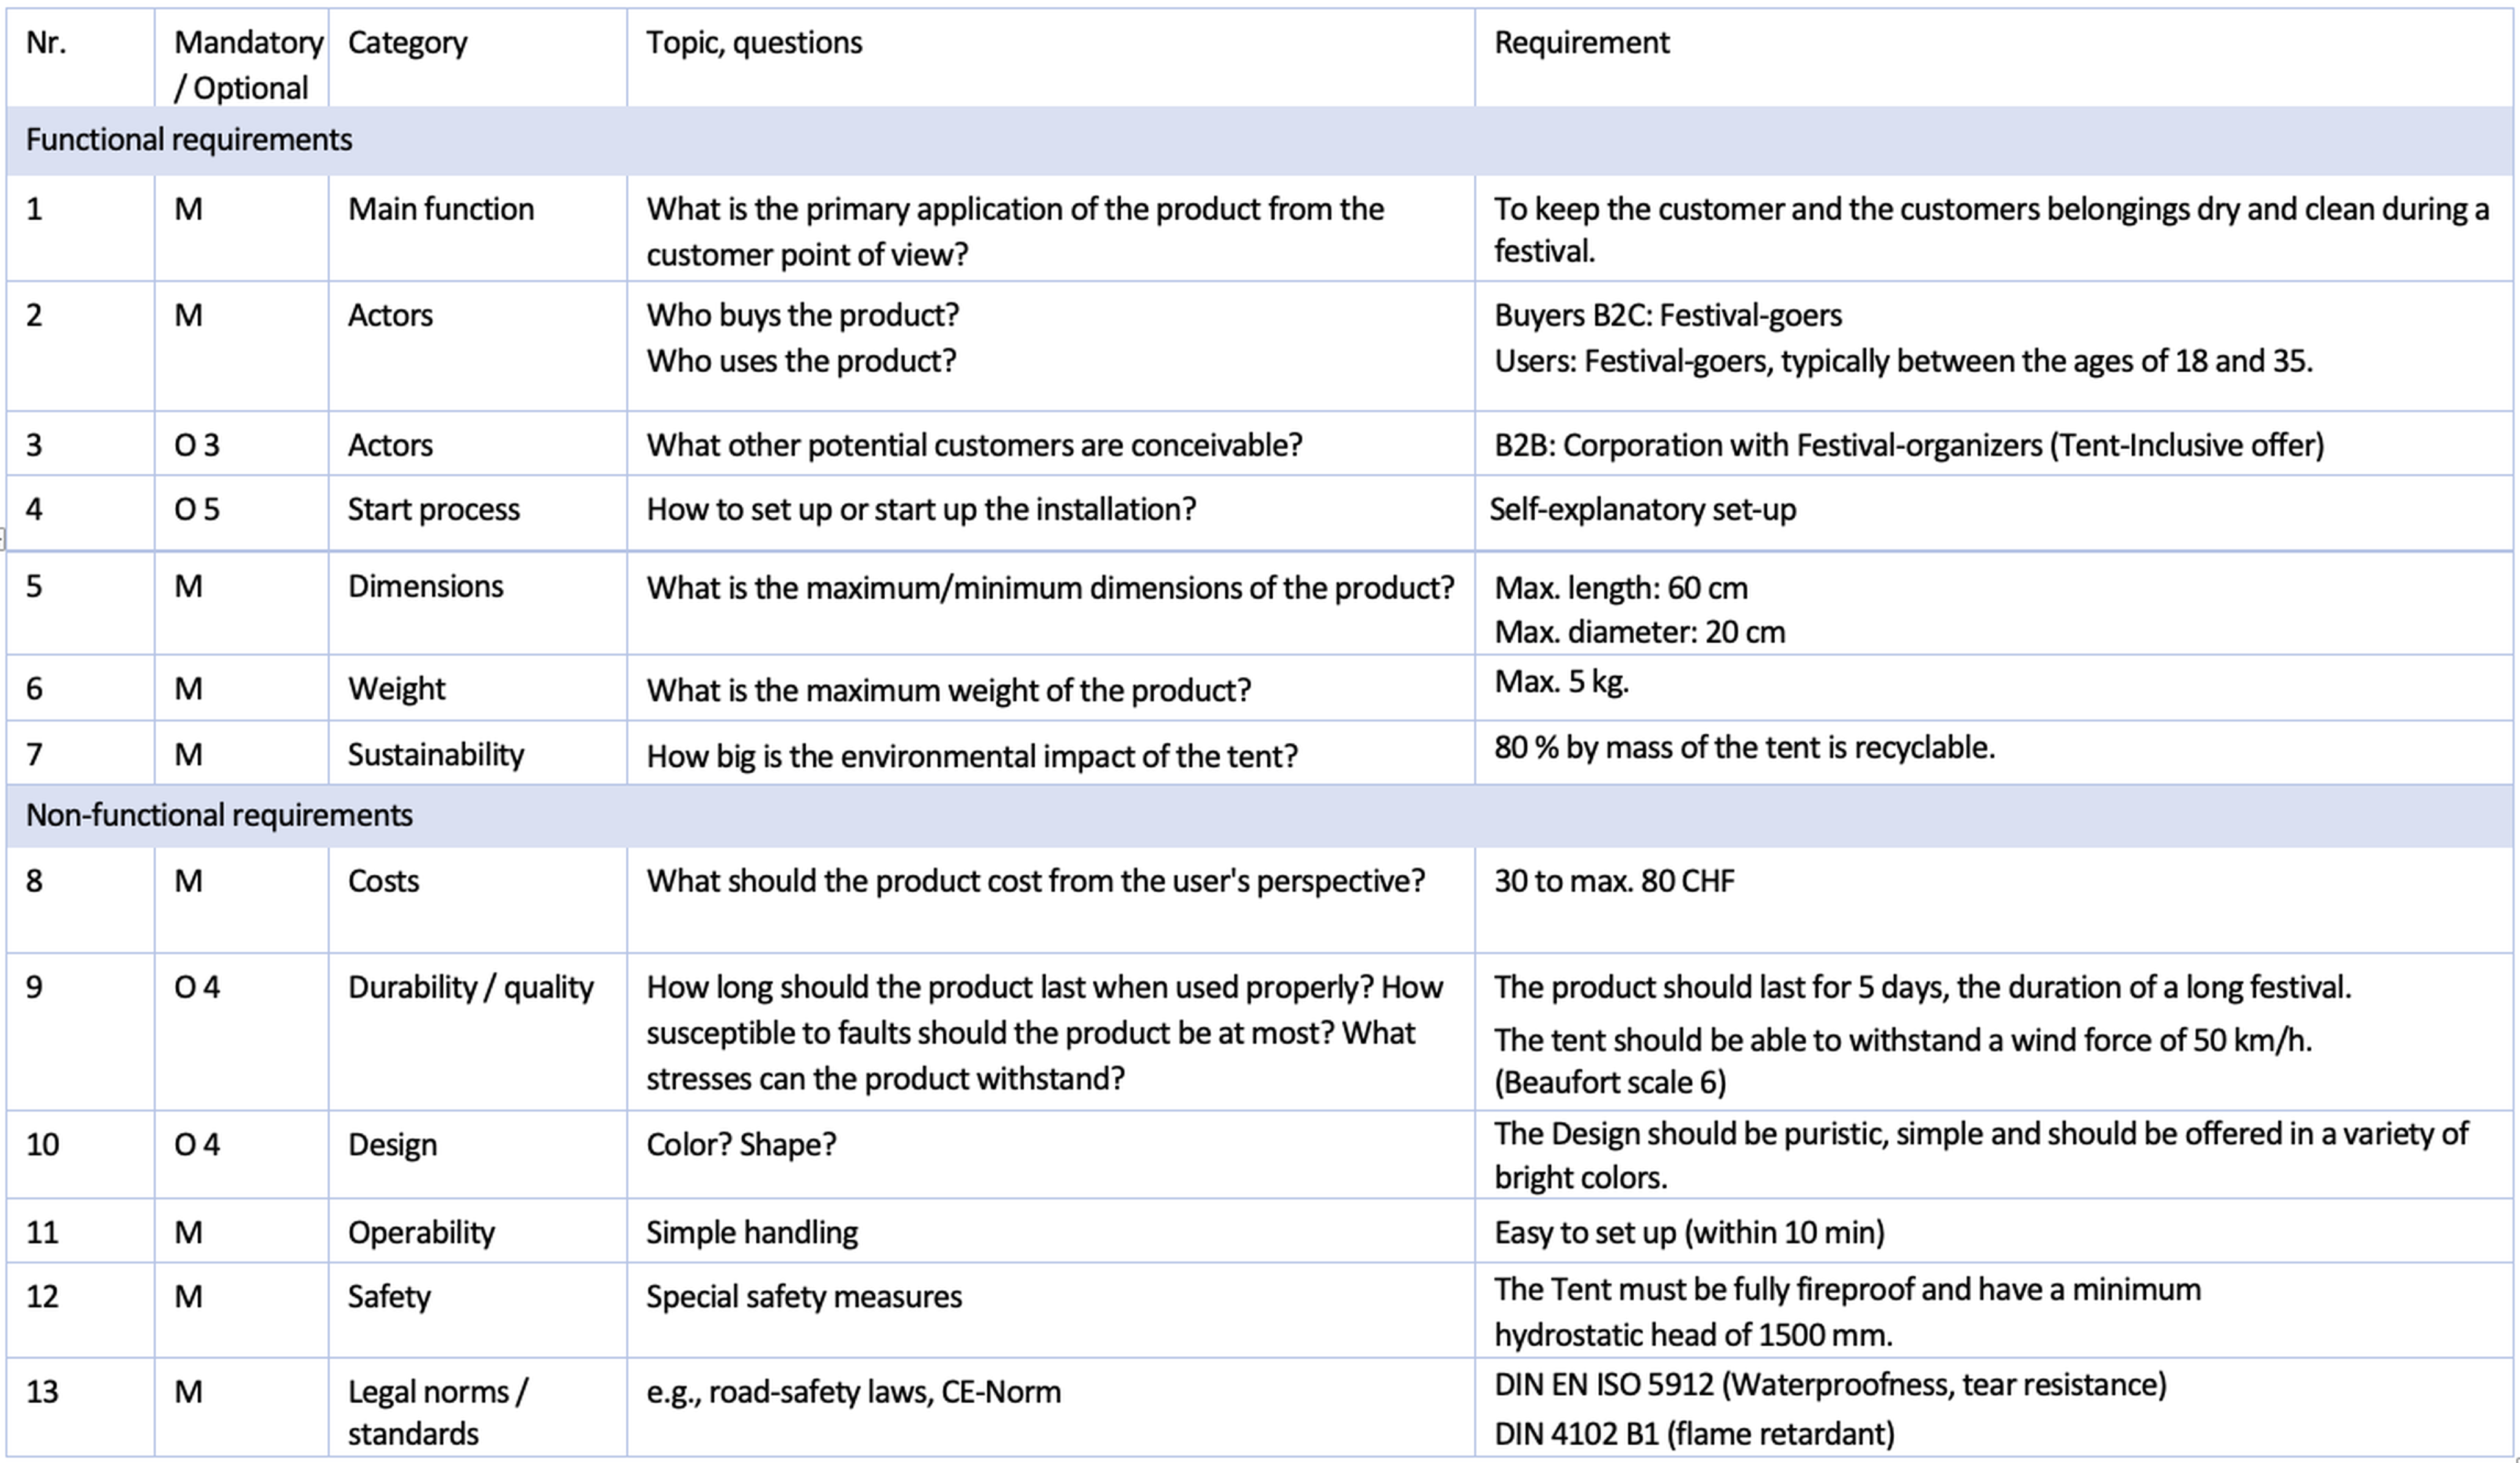
\includegraphics[width=\textwidth]{media/req_cat_high_res.png}
    \label{tab:cat_of_req}
\end{table}

\subsection{Morphological box}
This chapter describes the process of developing three design variants for a sustainable
festival tent using the morphological box method. The product was divided into key
subproblems, such as shape, size, structure support, lifespan, and material processing.
For each subproblem, a range of possible solutions was researched, resulting in the
initial morphological box (\autoref{sec:appendix}, \autoref{tab:initial_morph}).

To streamline the process, less critical subfunctions, like color, design and
biodegradation duration, were excluded, and unsuitable materials, such as unprocessed
MBCs and plastic, were removed. The refined
morphological box (\autoref{sec:appendix}, \autoref{tab:slimmed_morph}) formed the foundation
for selecting three promising design variants, which are detailed in \autoref{tab:morph_box}
and the following section. 

\begin{table}[ht!]
    \centering
    \caption{Morphological box with three solution variants}
    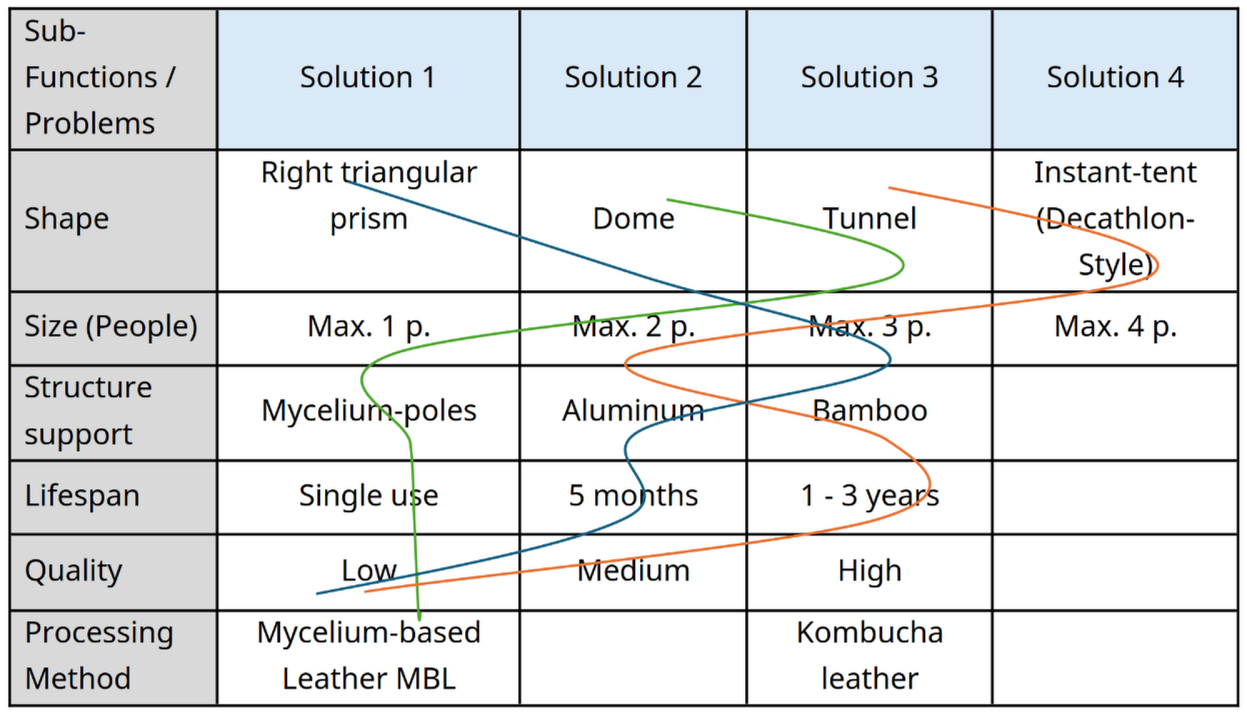
\includegraphics[width=.85\textwidth]{media/morph_box.png}
    \label{tab:morph_box}
\end{table}

\subsubsection{Description of the three solution variants}
\pph{\color{newgreen}{Variant 1: Dome tent (Single use, Fully biodegradable)}}
The first variant is a dome-shaped tent, constructed entirely from biodegradable materials,
including mycelium poles and Mycelium-Based Leather (MBL). This variant is designed for
single-use and aims to provide the highest possible grade of biodegradability. It is produced
with a focus on low-cost and low-quality materials, suitable for short-term use at festivals.

\pph{\color{neworange}{Variant 2: Tunnel tent (Four-person, Long-lasting)}}
The second variant is a tunnel tent, chosen for its optimal space-to-weight ratio, making it
suitable for accommodating four people—the largest capacity in this selection. It is designed
with higher-quality materials for a lifespan of one to three years, supported by an aluminum
structure for enhanced durability and stability.

\pph{\color{newblue}{Variant 3: Triangular prism tent (Two-person, Medium-lasting)}}
The third variant is a right triangular prism-shaped tent, designed for two people. This option
combines features from both the high-quality tunnel tent and the single-use dome tent. It
uses bamboo poles, which provide greater longevity than mycelium but are less durable
than aluminum, while still maintaining biodegradability.

The final selection between these three variants will be made in the following chapter.

\subsection{Value-Benefit analysis}
\autoref{tab:val-ben} presents the Value-Benefit analysis of the three previously described tent variants. In
alignment with our primary objective of addressing plastic waste at festivals, recyclability is
assigned the highest priority. The affordability of each variant is also crucial, as it must remain
competitive with existing products that contribute to the plastic waste problem. Given that
the target market is festival-goers seeking short-term, disposable solutions, the overall quality
and lifespan of the tents are less critical, as the aim is not to compete in the
high-quality tent market.

The analysis includes a row for ``Weather Resistance'', which evaluates the tent's ability to
endure adverse weather conditions, such as heavy winds. This aspect is particularly relevant
as different shapes provide varying levels of structural resilience.

\begin{table}[ht!]
    \centering
    \caption{Value-Benefit analysis}
    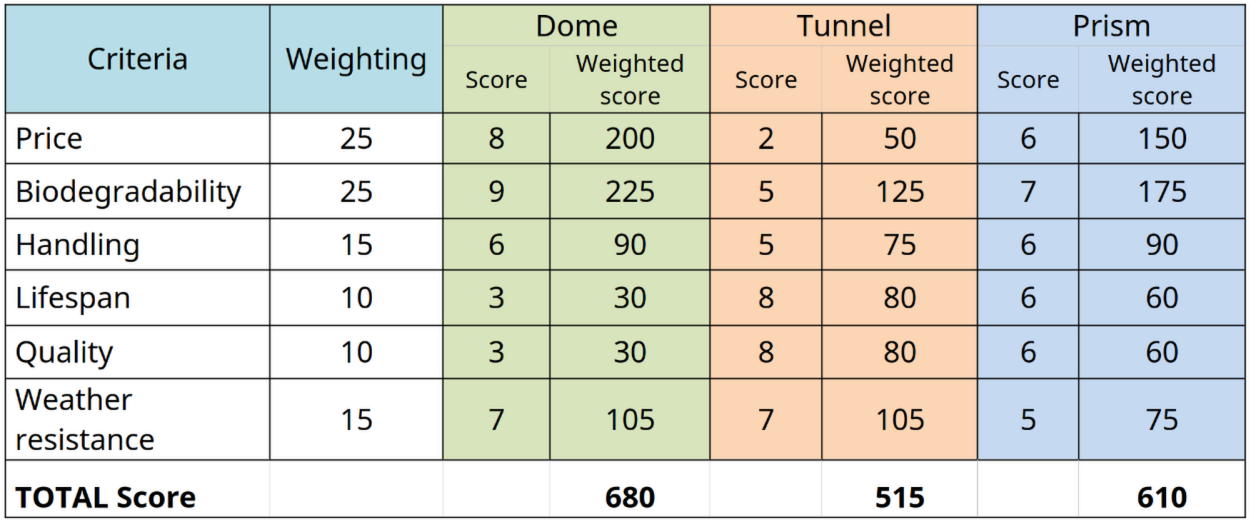
\includegraphics[width=.85\textwidth]{media/val-ben.png}
    \label{tab:val-ben}
\end{table}

\subsubsection{Justified choice}
Based on the weighted ratings derived from the Value-Benefit analysis (\autoref{tab:val-ben}),
the Dome Tent variant emerges as the most suitable option, achieving a total score of 680
points, the highest among all variants. This reflects its strong alignment with customer
requirements, such as affordability, ease of use, and reduced environmental impact,
making it particularly appealing to festival-goers. Its features address key customer
needs for sustainable temporary shelter, while effectively contributing to the goal of
reducing plastic waste in festival environments.

\section{Final concept}
\label{sec:final_concept}
This chapter presents the finalized \myc\ design, detailing its structure, key features,
and components. It provides technical specifications based on the concept and includes
plans and diagrams for fabrication and assembly.

\subsection{Product concept}
This section presents an overview of the \myc, detailing its features with labelled
images of a simplified model that illustrates the structure and key components.

\begin{figure}[ht!]
    \centering
    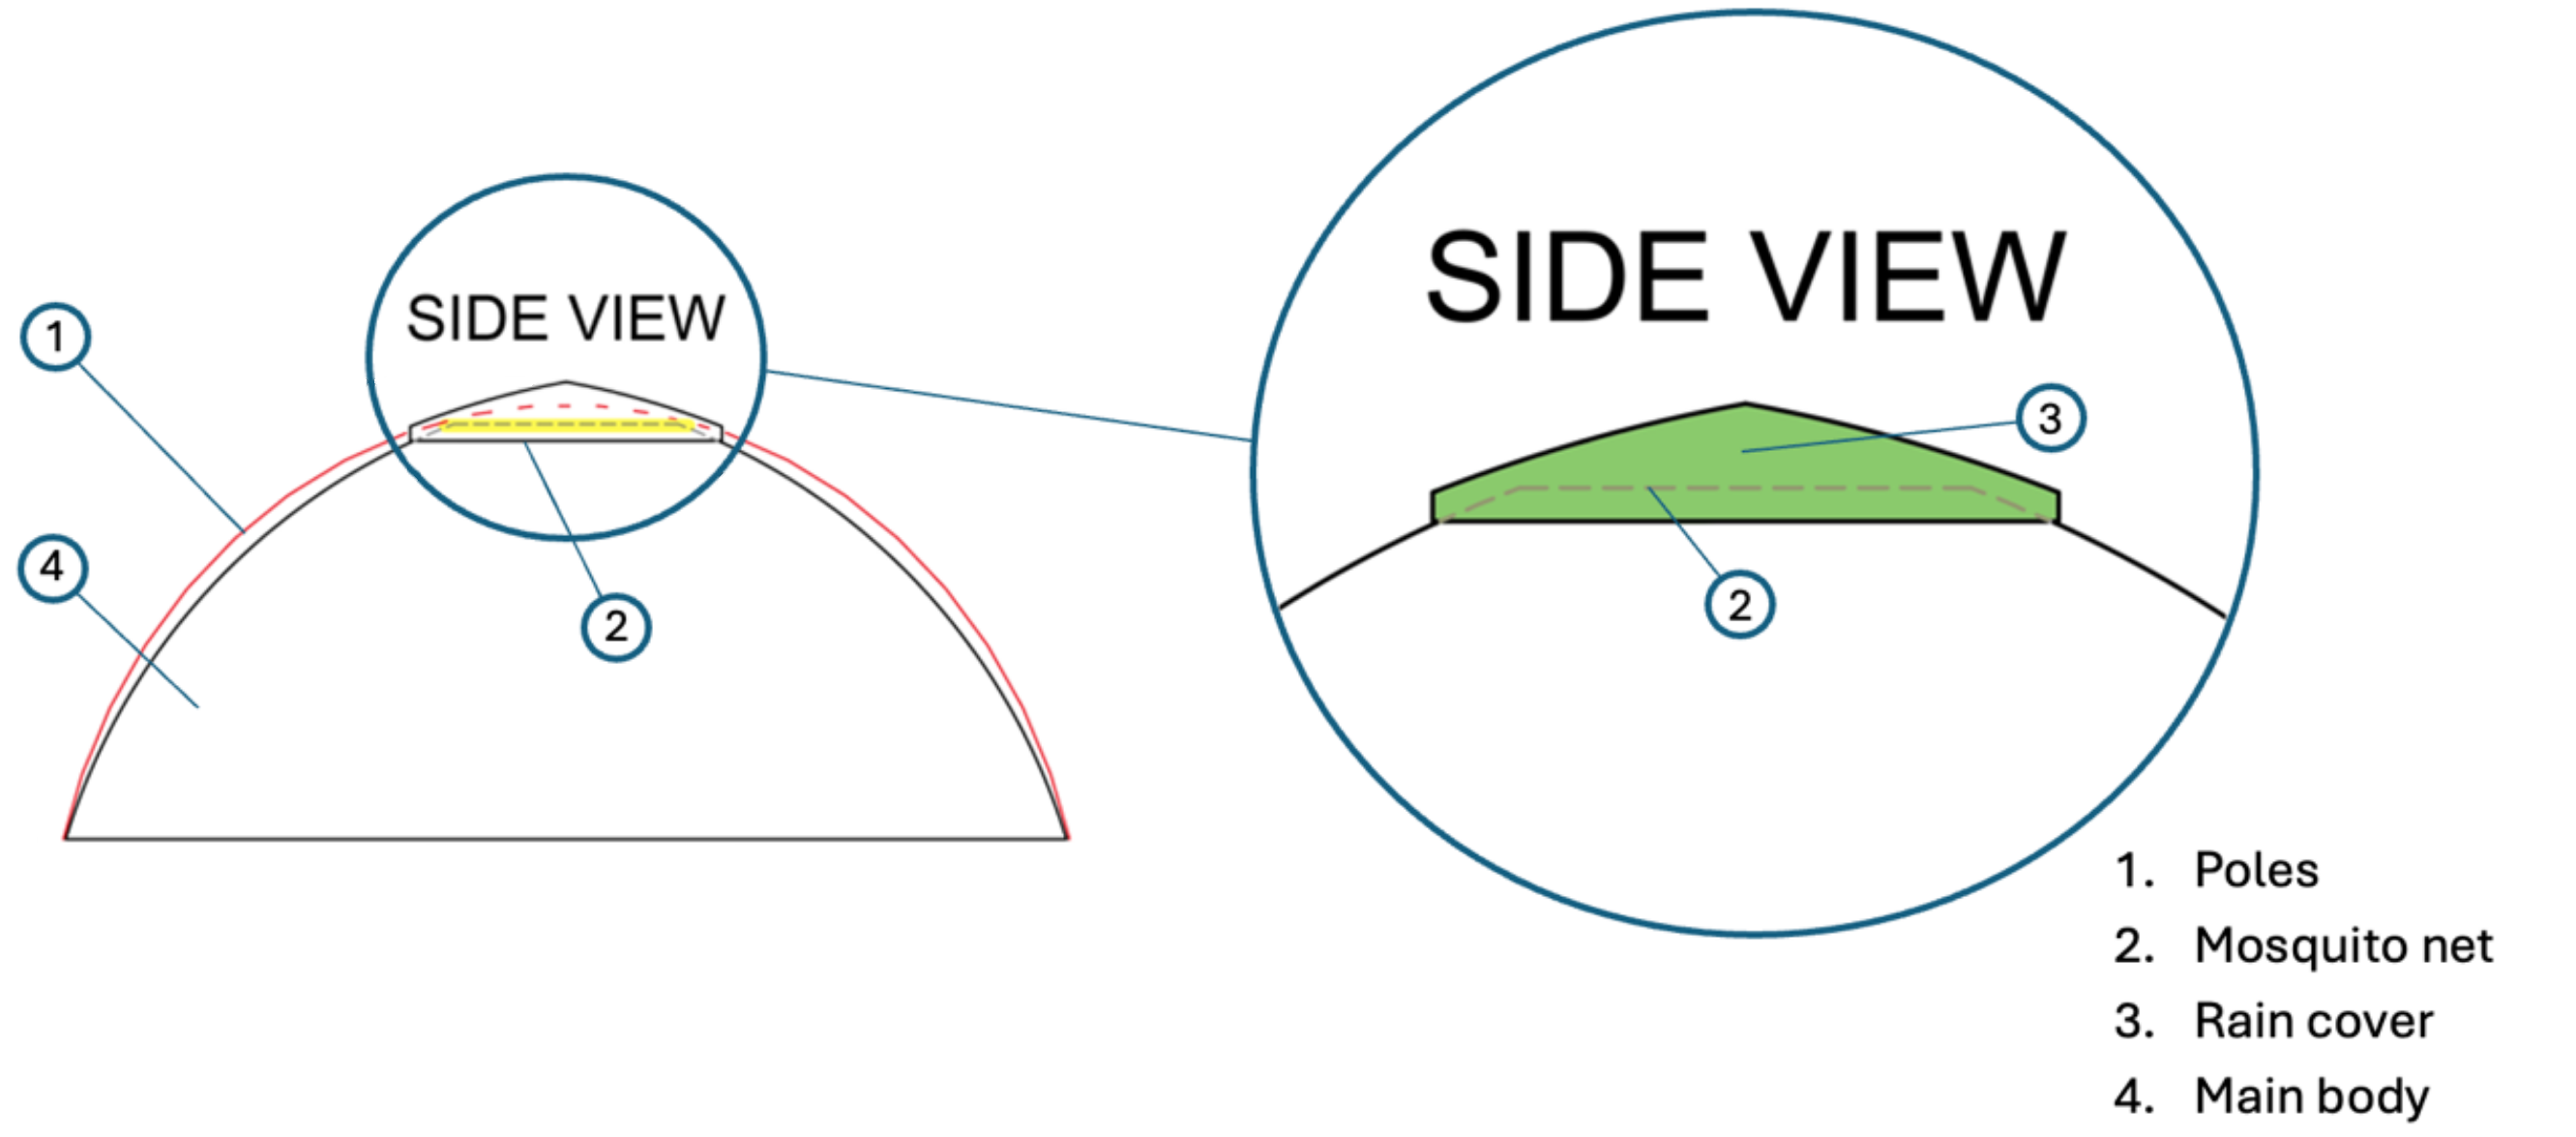
\includegraphics[width=.85\textwidth]{media/side_view.png}
    \caption{Details side view}
    \label{fig:side_view}
\end{figure}

The main body of the tent is fully enclosed, extending up to the top, where an opening with a
protective mosquito net ensures constant air circulation. This ventilation opening is
safeguarded by a rain cover to prevent water ingress while allowing airflow. To maintain an
optimal space between the tent body and the rain cover, the tent poles are positioned
externally, supporting the rain cover above the body. This structure is depicted in \autoref{fig:side_view}

\newpage
\begin{figure}[ht!]
    \centering
    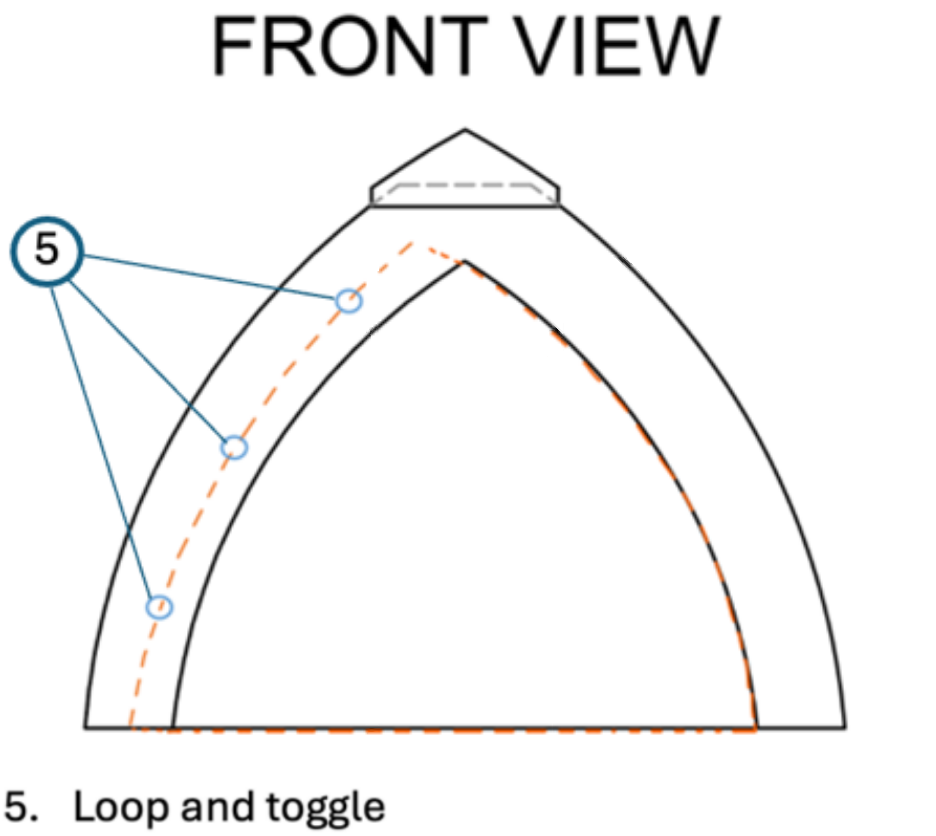
\includegraphics[width=.35\textwidth]{media/front_view.png}
    \caption{Details side view}
    \label{fig:front_view}
\end{figure}

Entry to the tent is facilitated by a secure loop-and-toggle system. Additionally, the
door features an overlapping design to prevent rain from entering the tent, as shown by
the orange line in \autoref{fig:front_view}.

\subsection{Technical specifications}
The technical specifications display the list of the main components such as size and
material in \autoref{tab:tech_spec}. These specifications are based on the features laid
out in the conception of product \autoref{sec:final_concept} and the morphological box.

The intention of the single use tent translates into biodegradable tent materials. However,
this criteria for the accessories shown in \autoref{tab:tech_spec} cannot be fulfilled at this stage of
development.

\begin{table}[ht!]
    \caption{Technical specifications}
    \label{tab:tech_spec}
    \begin{tabularx}{\textwidth}{|>{\raggedright\arraybackslash}p{3cm}|>{\raggedright\arraybackslash}p{2.5cm}|>{\raggedright\arraybackslash}p{2.5cm}|>{\raggedright\arraybackslash}p{2cm}|>{\raggedright\arraybackslash}X|}
    \hline
    \rowcolor[gray]{0.75}
    \textbf{Description} & \textbf{Material} & \textbf{Size in cm} & \textbf{Pieces} & \textbf{Notes} \\
    \hline
    Bottom part & Mylo leather & 215 x 215 & 1 & Floor plan +30cm \\
    \hline
    Poles & Mycelium & 324 & 2 & \\
    \hline
    Rain cover & Mylo leather & 65 x 65 & 1 & \\
    \hline
    Cover (main body) & Mylo leather & 185 x 150 & 4 & \\
    \hline
    Latch & Cotton & & & Velcro has no biodegradable product on the market yet\\
    \hline
    Rope / cord & Jute & 200 & 2 & \\
    \hline
    Perforated net & Mycelium mash & \diameter 65 & 1 & \\
    \hline
    \multicolumn{5}{|p{.973\textwidth}|}{\cellcolor[gray]{0.75}\textbf{Accessories}} \\ 
    \hline    
    Peg & Aluminium & & 8 & \\
    \hline
    \end{tabularx}
\end{table}

\subsection{Construction plans}
The construction plans show in detail the shape and size of the tent. The final product
will be based on these technical plans, as well as its components will depend on them.
The tent consists of two main elements: the tent itself and the airtight cap.

The structure of the \myc\ is made from mycelium, as is the access door.
Its base measures (LxW) 185x185 cm, while the height from the base to the highest point (H)
is 140 cm as shown in \autoref{sec:appendix}, \autoref{pdf:tent-size} (Tent size).\\
It has a central circular hole on the highest part, which promotes optimal air exchange
and the passage of natural light.

Together with the circular hole, a fine mycelium perforated net is provided to supply
protection against all kinds of insects. It is also designed to facilitate night vision for starry
sky observers.

The airtight cap is also made from mycelium. Its main feature is that it is mountable at
any time and serves to prevent water or too much sunlight from entering the interior of
the tent. The cap is also raised to always ensure air exchange inside the tent.

The dimensions of the circular cap are \diameter 60cm, and circumference 188.5 cm
as shown in \autoref{sec:appendix}, \autoref{pdf:tent-size} (Tent size).
The cap is placed on the tent poles and tied to them.

The \myc\ with the mounted cap measures (LxWxH) 185x185x\~150 cm.

\section{Mock-up}
The mock-up presentation is a key part of the project, allowing users to visualize and
understand the tent's design. The tent's features, including the removable cap and door
operation with the respective materials used to create the mock-up, will be shown below.

\subsection{Concept of mock-up}
The \myc\ mock-up (\autoref{fig:final_mockup}) serves as a scaled-down representation of
the full-size product, designed to demonstrate its key features in a compact form. With
dimensions of (LxWxH) 17.5x17.5x14 cm, the mock-up reflects the core functional and
structural elements of the actual tent, offering a conceptual demonstration of its design
principles.

\subsubsection{Key featues}
The mock-up includes a fully enclosed body that replicates the real product’s upper
ventilation system, integrating a mosquito net and a rain cover to demonstrate airflow
and protective design. To showcase improved airflow and water resistance, external poles
are added and scaled to fit the smaller dimensions. The entry system is modeled to reflect
the functionality of the full-size tent, with a roll-and-button closure mechanism and
overlapping door design ensuring secure closure and rain protection.

\subsubsection{Purpose of the mock-up}
Despite its compact scale, the mock-up effectively highlights the design intent and
functionality of the MyceliumTent, serving as both a visual and structural reference for
its real-world counterpart.

\subsubsection{Material selection and design}
The final product will be constructed using mycelium, and a sample of this material is
exhibited alongside the mock-up (\autoref{fig:compact_myc}). Following the initial draft,
design adjustments were made to enhance both the shape and functionality of the model. The
construction process, detailed in \autoref{sec:appendix}, \autoref{pdf:mockup-size} (Mock-up size),
uses simple yet effective materials: cotton textiles for the rain cover and main body,
bronze metal string for structural framing, and mesh material for the mosquito net. These
components were carefully selected to align with the tent’s focus on sustainability and
environmental impact reduction.

\subsubsection{Mock-up pictures}
\begin{figure}[ht!]
    \centering
    \begin{minipage}{0.475\textwidth}
        \centering
        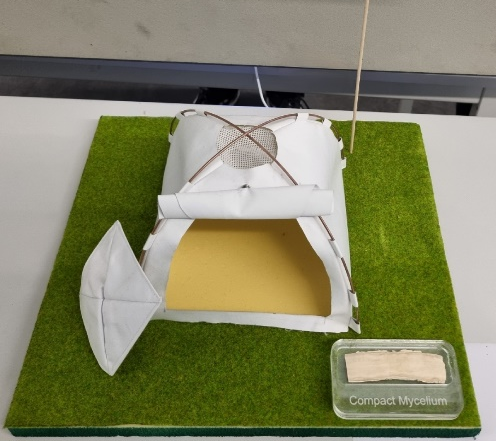
\includegraphics[width=.8\textwidth]{media/final_mockup.png}
        \caption{Final mock-up}
        \label{fig:final_mockup}
    \end{minipage}%
    \hfill
    \begin{minipage}{0.45\textwidth}
        \centering
        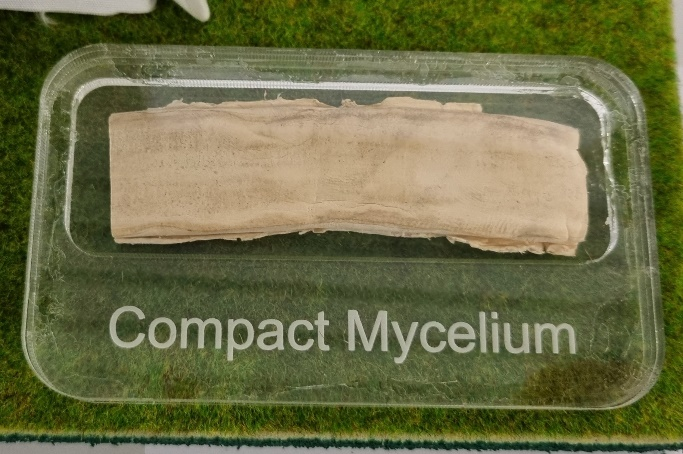
\includegraphics[width=\textwidth]{media/compact_myc.png}
        \caption{Sample of compact mycelium}
        \label{fig:compact_myc}
    \end{minipage}
\end{figure}

\newpage
\section{Testing}
This chapter examines the testing phase, which is critical to ensure that the product
meets technical specifications and fulfils customer requirements. The expected results
are then evaluated and further discussed in \autoref{sec:discussion}.

\subsection{Tests}
The testing process is divided into two principal areas: Verification and Validation. Each
are has three different tests listed. For every test the requirement, test procedure and
the expected result is described.

\subsubsection{Verification}
This subchapter discusses the verification process during the testing phase. The purpose of
this process is to ensure that the product has been developed correctly and meets the
predefined requirements.
Three of the most significant tests are outlined in \autoref{tab:verification}, with the
numbers in brackets indicating the corresponding links to the requirements catalogue (\autoref{tab:cat_of_req}).

\renewcommand{\arraystretch}{1.5}

\begin{table}[ht!]
    \caption{Verification tests}
    \label{tab:verification}
    \begin{tabularx}{\textwidth}{|>{\raggedright\arraybackslash}p{2.5cm}|>{\raggedright\arraybackslash}p{3.5cm}|>{\raggedright\arraybackslash}p{6cm}|>{\raggedright\arraybackslash}X|}
    \hline
    \rowcolor[gray]{0.75}
    \textbf{Function} & \textbf{Requirement} & \textbf{Test procedure} & \textbf{Expected Result} \\
    \hline
    Hydrostatic head (1/12) & 
    The tent should have a minimum hydrostatic head of 1500 mm & 
    The hydrostatic head is determined by a water pressure test. The material is subjected to increasing water pressure. This continues until the material allows water to pass through. When the third drop has penetrated to the other side, the test ends. &
    The height of the water column at the point of water passage is above 1500 mm. $\mathbf{\Rightarrow}$\textcolor{newgreen}{\textbf{Fulfilled}} \\
    \hline
    Wind resistance (9) &
    The tent should be able to withstand a wind force of 50 km/h (Beaufort scale 6). &
    The tent is set up on a meadow and tested with a wind generator simulating a wind speed of 50 km/h for 30 minutes. Inside, it contains a sleeping bag, sleeping mat, and backpack with a total weight of 8 kg. The meadow has a minimum soil moisture of 40\%, reflecting conditions after rainfall. This worst-case scenario eliminates the need for additional tests, as drier conditions improve results. &
    The tent remains in place for half an hour. $\mathbf{\Rightarrow}$\textcolor{newgreen}{\textbf{Fulfilled}} \\
    \hline
    Air circulation (1) &
    It is not only the waterproofness that determines whether it stays dry inside the tent. The geometry of the tent must allow the humidity to be transported outside. &
    A humidifier is placed in the tent and switched on for 8 hours. It is set to release 50 ml of water per hour, which is roughly equivalent to a human being breathing. At the same time, the wind generator is set to 20 km/h to simulate a realistic wind situation on a large field. &
    No water collects on the tent floor after 8 hours: $\mathbf{\Rightarrow}$\textcolor{newgreen}{\textbf{Fulfilled}} \\
    \hline
    \end{tabularx}
\end{table}

\newpage
\subsubsection{Validation}
This subchapter outlines the validation process, which involves three key tests
(\autoref{tab:validation}) o determine whether the correct product has been developed
and whether it fulfills customer requirements as specified in the requirements catalog. The
aspects evaluated include the operability, sustainability, and durability of the tent during a
festival. As all requirements are mandatory, each test must be successfully validated to ensure
compliance.

\begin{table}[ht!]
    \caption{Validation tests}
    \label{tab:validation}
    \begin{tabularx}{\textwidth}{|>{\raggedright\arraybackslash}p{2.5cm}|>{\raggedright\arraybackslash}p{3.5cm}|>{\raggedright\arraybackslash}p{6cm}|>{\raggedright\arraybackslash}X|}
    \hline
    \rowcolor[gray]{0.75}
    \textbf{Function} & \textbf{Requirement} & \textbf{Test procedure} & \textbf{Expected Result} \\
    \hline
    Operability (4/11) & 
    The set-up of the tent should be self-explanatory and fully constructed in 10 minutes. & 
    20 subjects aged between 18 and 35, who have no physical impairments, each get 10 minutes to completely set up the tent. The only aid they are given is a construction manual, with a visual and written demonstration of the set-up process. &
    All 20 subjects are expected to fully set up the tent within the given timeframe. $\mathbf{\Rightarrow}$\textcolor{newgreen}{\textbf{Fulfilled}} \\
    \hline
    Sustainability (7) &
    80\% by mass of the tent should be recyclable. &
    The mass of the recyclable parts of the tent are added and compared to the tent’s complete mass to determine the percentage of the recyclable material. &
    Due to insufficient details on the density of MBL only an assumption can be made. However, considering the fact, that the only non-recyclable components are the pegs, it is expected that more than 80\% of the total mass is recyclable. $\mathbf{\Rightarrow}$\textcolor{newgreen}{\textbf{Fulfilled}} \\
    \hline
    Durability during a Festival (1) &
    The tent should keep the customers and their belongings dry and clean. &
    During a five-day festival, the tent will be put to normal use by a subject in a simulation of the unexpected incidents or weather changes than can appear during a festival. The test will be conducted during a period, when rain is guaranteed. Therefore, if a festival concludes with no rainfall, the test shall be repeated at a different festival. This process will be repeated until rainfall has occurred. &
    The tent is expected to withstand the five day festival and keep the belongings and the subject themself dry and clean. $\mathbf{\Rightarrow}$\textcolor{newgreen}{\textbf{Fulfilled}} \\
    \hline
    \end{tabularx}
\end{table}

The use of the fully developed mycelium-based material is crucial for the tests outlined
in this subchapter. Since a mock-up does not accurately represent the material's
properties and behaviour in its final form, these tests must instead be conducted using
the first prototype, which incorporates the fully developed material. This approach
ensures that the material performance, durability, and sustainability can be assessed in
real-world conditions, providing reliable data for further development and refinement of
the product.

\subsection{Discussion}
\label{sec:discussion}
Regarding the verification tests, the primary source of uncertainty lies in the water resistance
of the material, particularly its water column. Existing materials with adequate water
resistance, such as alternatives to rubber seals (\autoref{fig:compact_myc}), demonstrate
that it is feasible to produce a mycelium-based material with similar properties. Nevertheless,
further testing is required to determine whether the material maintains its water
resistance at very thin wall thicknesses, which is crucial for meeting weight specifications.

Wind resistance is unlikely to pose a significant challenge due to the aerodynamic, wind-slip
shape of the tent. However, the ability to effectively manage moisture inside the tent remains
a concern. As this is a single-wall design, the construction and shape of the tent play a critical
role in facilitating ventilation. To address this, the ventilation opening has been enlarged
relative to the tent's total surface area. The effectiveness of this design will only become clear
during prototype testing.

Like the wind resistance, the validated operability and sustainability are unlikely to cause later
complications. This is due to the fact that the tent not only has a simple structure and a
construction manual as an available aid for the set-up process but is also made predominantly
out of a recyclable and biodegradable material. The overall durability of the tent during a
festival on the other hand could lead to further concern. Additional tests during extended
festivals with varying weather conditions will need to be performed to clarify how well the
tent can withstand longer and more challenging conditions.

\section{Conclusion}
The \myc\ project has sought to address the critical environmental issue of waste
accumulation at festivals by developing a tent composed of a fully sustainable and recyclable
material. Mycelium, characterized by its high recyclability and cost-efficient cultivation, has
shown promise as a potential solution. However, a key challenge remains the evaluation of its
suitability as a tent material. Addressing this challenge requires extensive research and
development, which falls beyond the scope of this project.

Despite these challenges, the concept has demonstrated substantial potential. It responds to
an urgent environmental problem and offers a compelling business opportunity, particularly
as a B2B solution for festival operators. Collaborations with such stakeholders could
significantly enhance the project's impact and feasibility.

Future work should prioritise comprehensive research into the material properties of
mycelium, followed by the production and evaluation of prototypes under realistic
conditions. This iterative development process will enable the refinement of the
product to ensure its functionality and durability. Given the significance of the problem
and the potential of the proposed solution, continuation of this project is strongly
recommended.

\newpage
\pagestyle{empty}
\section{Appendix}
\subsection{Declarations on the use of AI tools}
\begin{itemize}
    \item \textit{DeepL} and \textit{ChatGPT 4o} have been used as a spell-checker;\\
        \url{https://www.deepl.com/}\\
        \url{https://www.chatgpt.com/}
\end{itemize}

\subsection{Lists and references}

\listoftables

\listoffigures

\setlength{\bibitemsep}{1.2\baselineskip}
\printbibliography

%\newpage
%\begin{landscape}
%    \thispagestyle{empty}
%    \label{sec:appendix}
%    \begin{table}[ht!]
%        \centering
%        \caption{Appendix table}
%        \label{tab:appendix}
%        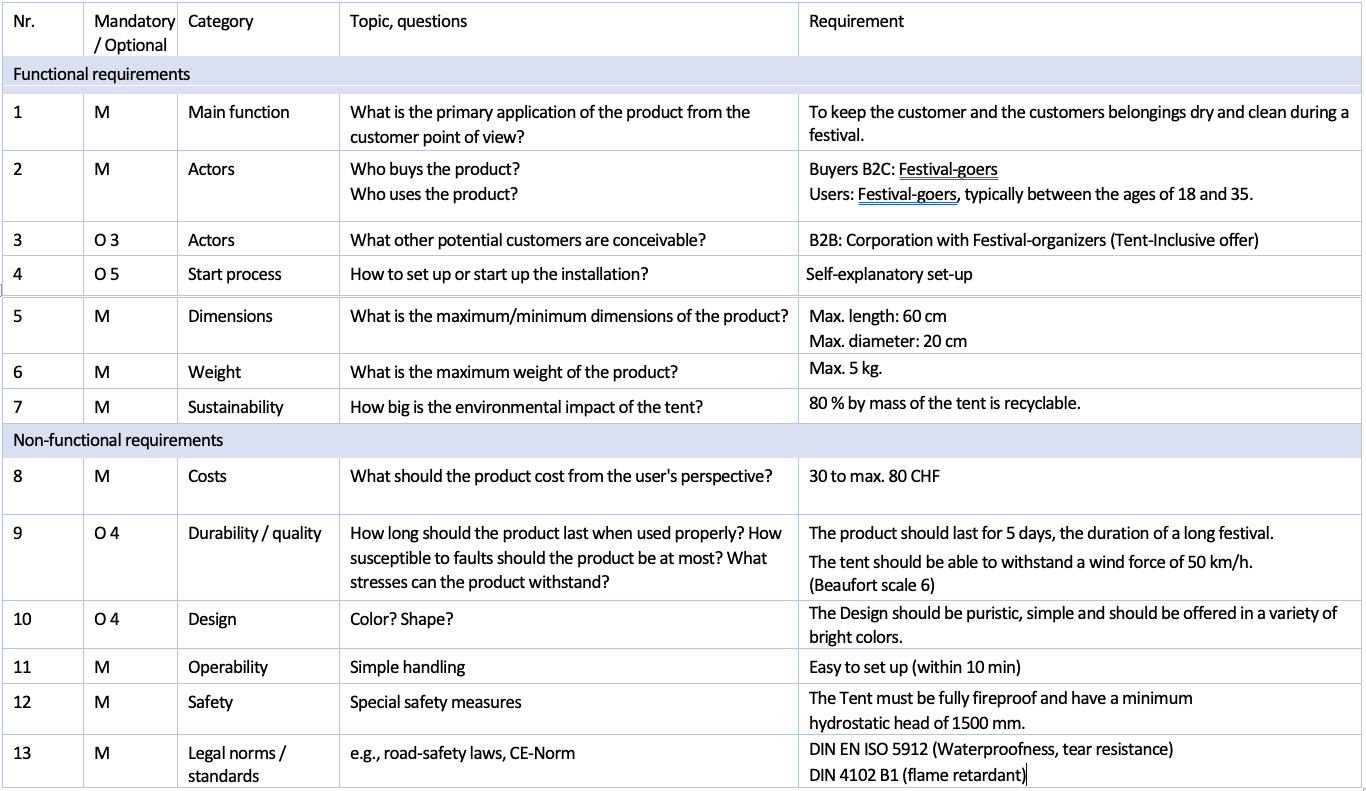
\includegraphics[width=1.5\textwidth]{media/appendix.png}
%    \end{table}
%\end{landscape}

\newpage
\section{Attachments}
\pagestyle{fancy}
\begin{table}[ht!]
    \centering
    \caption{Appendix: Initial morphological box}
    \label{tab:initial_morph}
    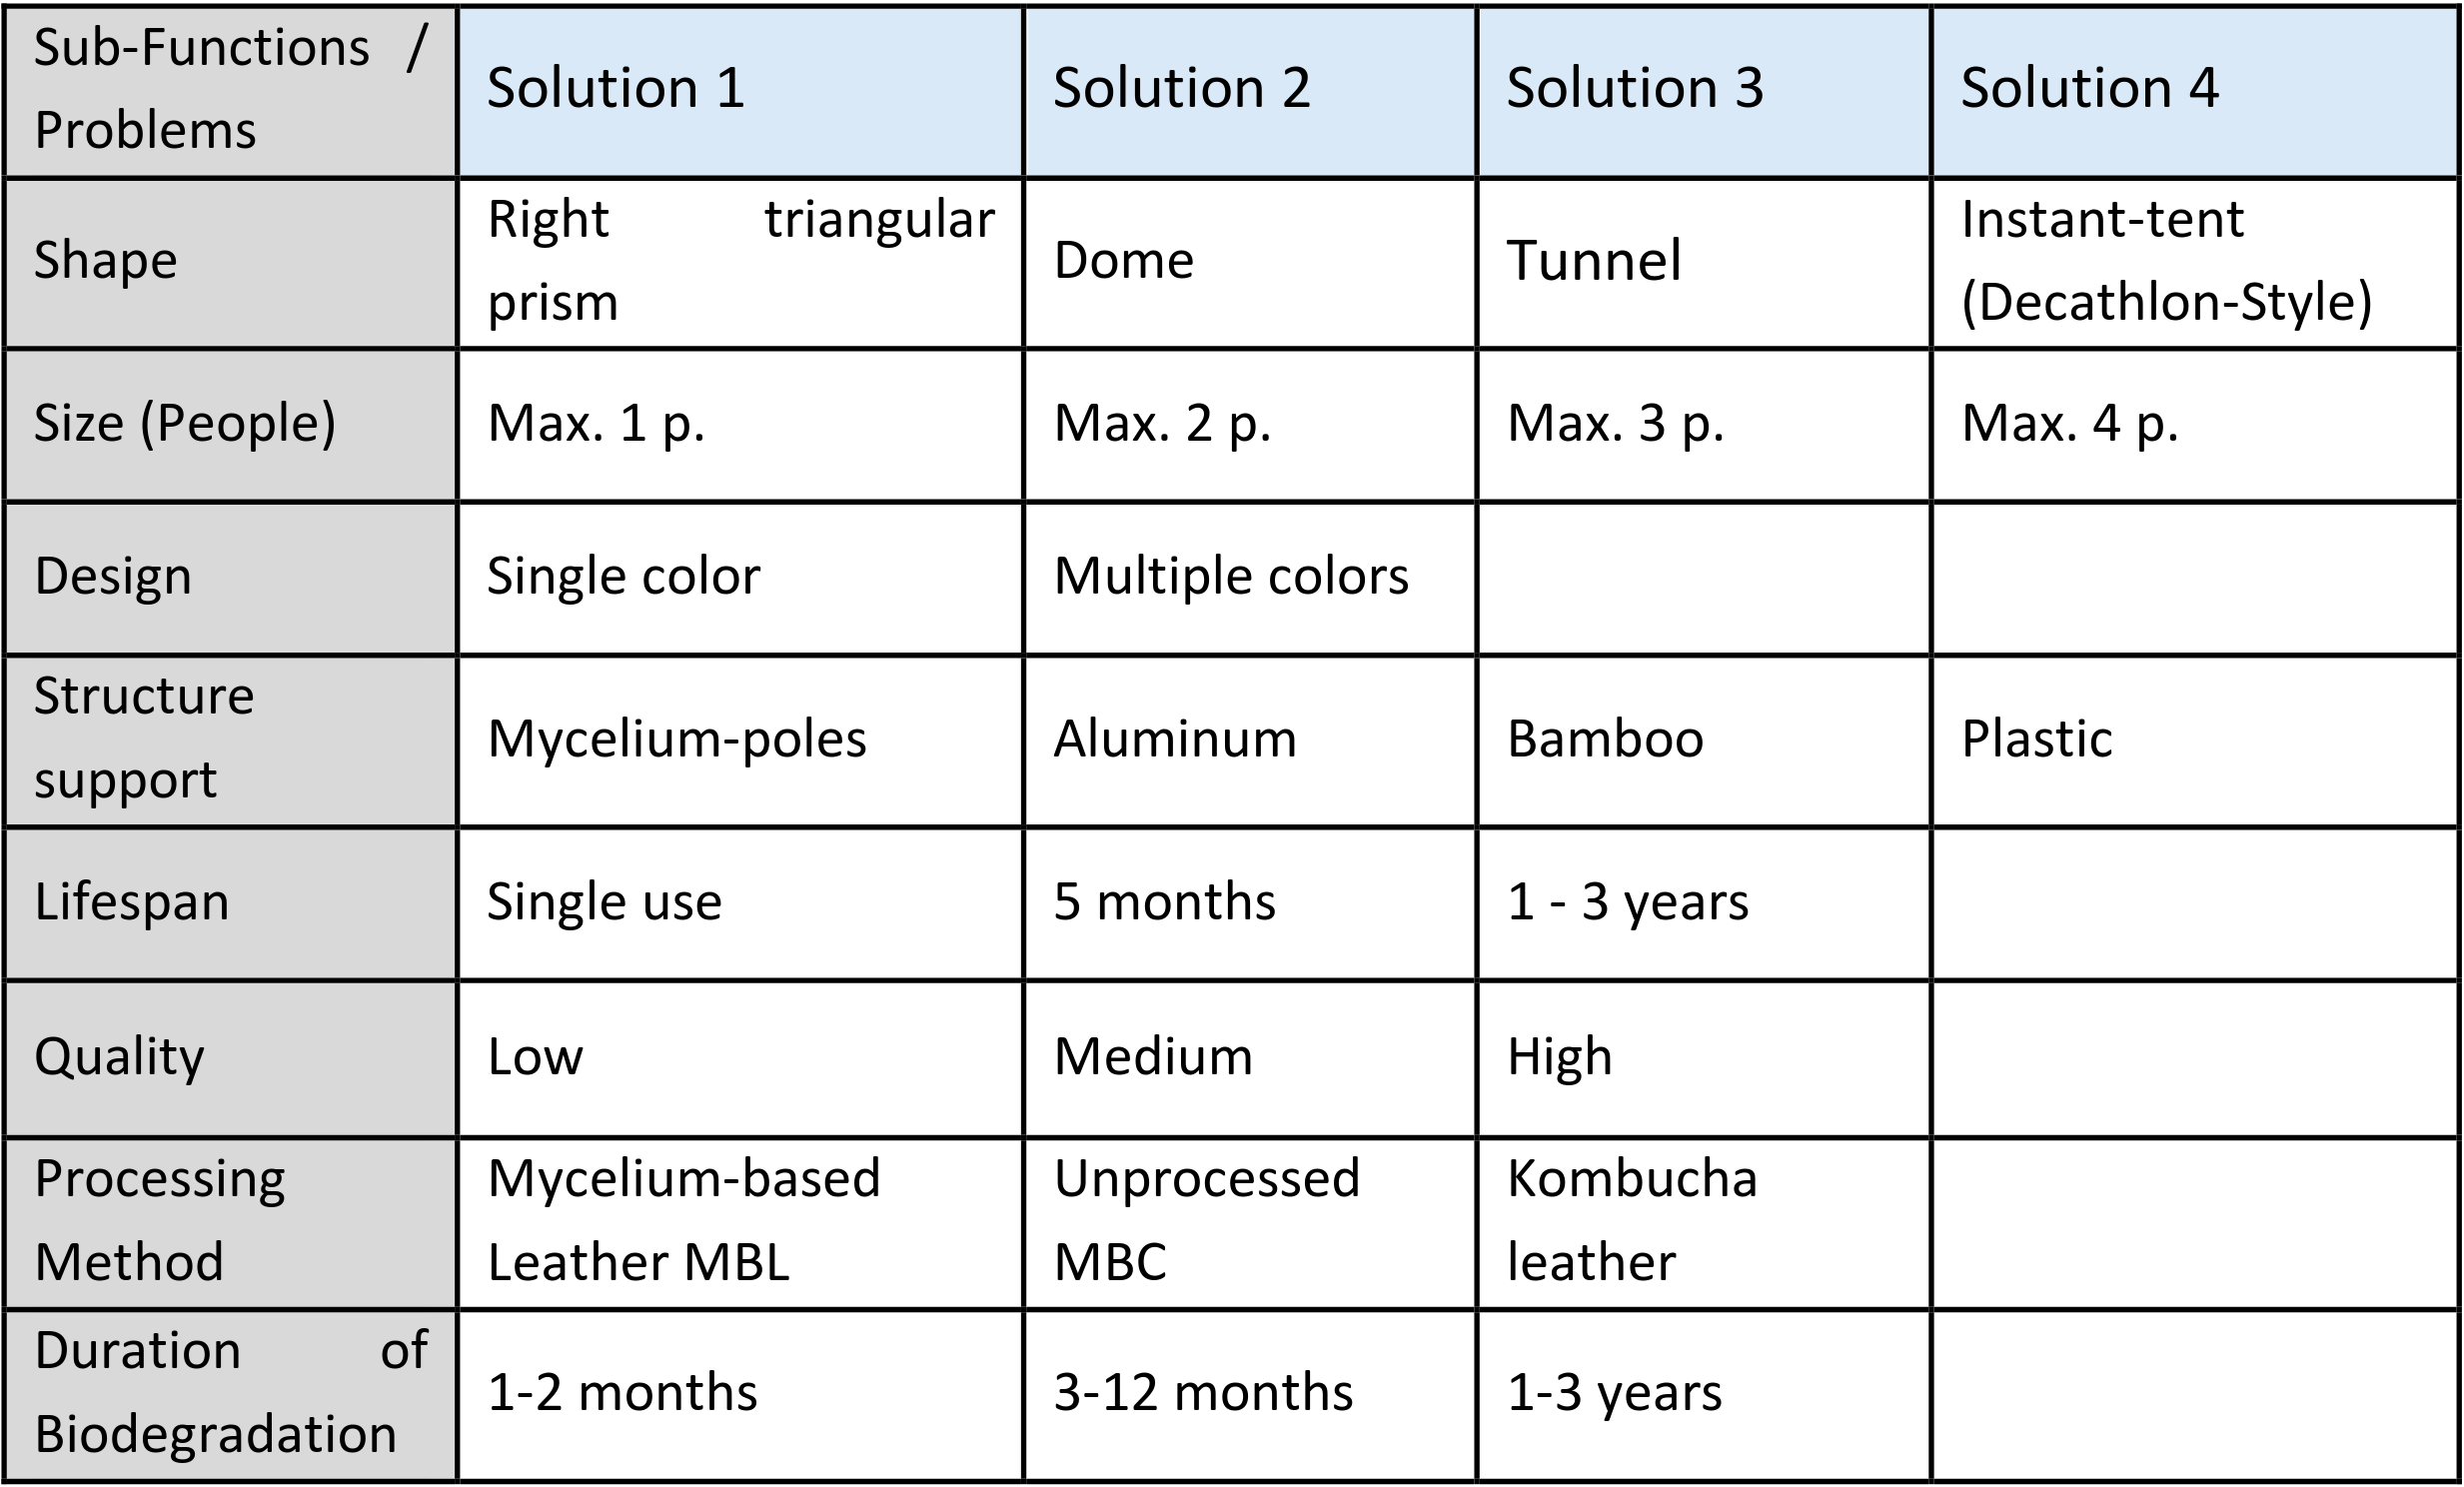
\includegraphics[width=\textwidth]{media/initial_morph.png}
\end{table}

\vfill
\begin{table}[ht!]
    \centering
    \caption{Appendix: Slimmed-down morphological box}
    \label{tab:slimmed_morph}
    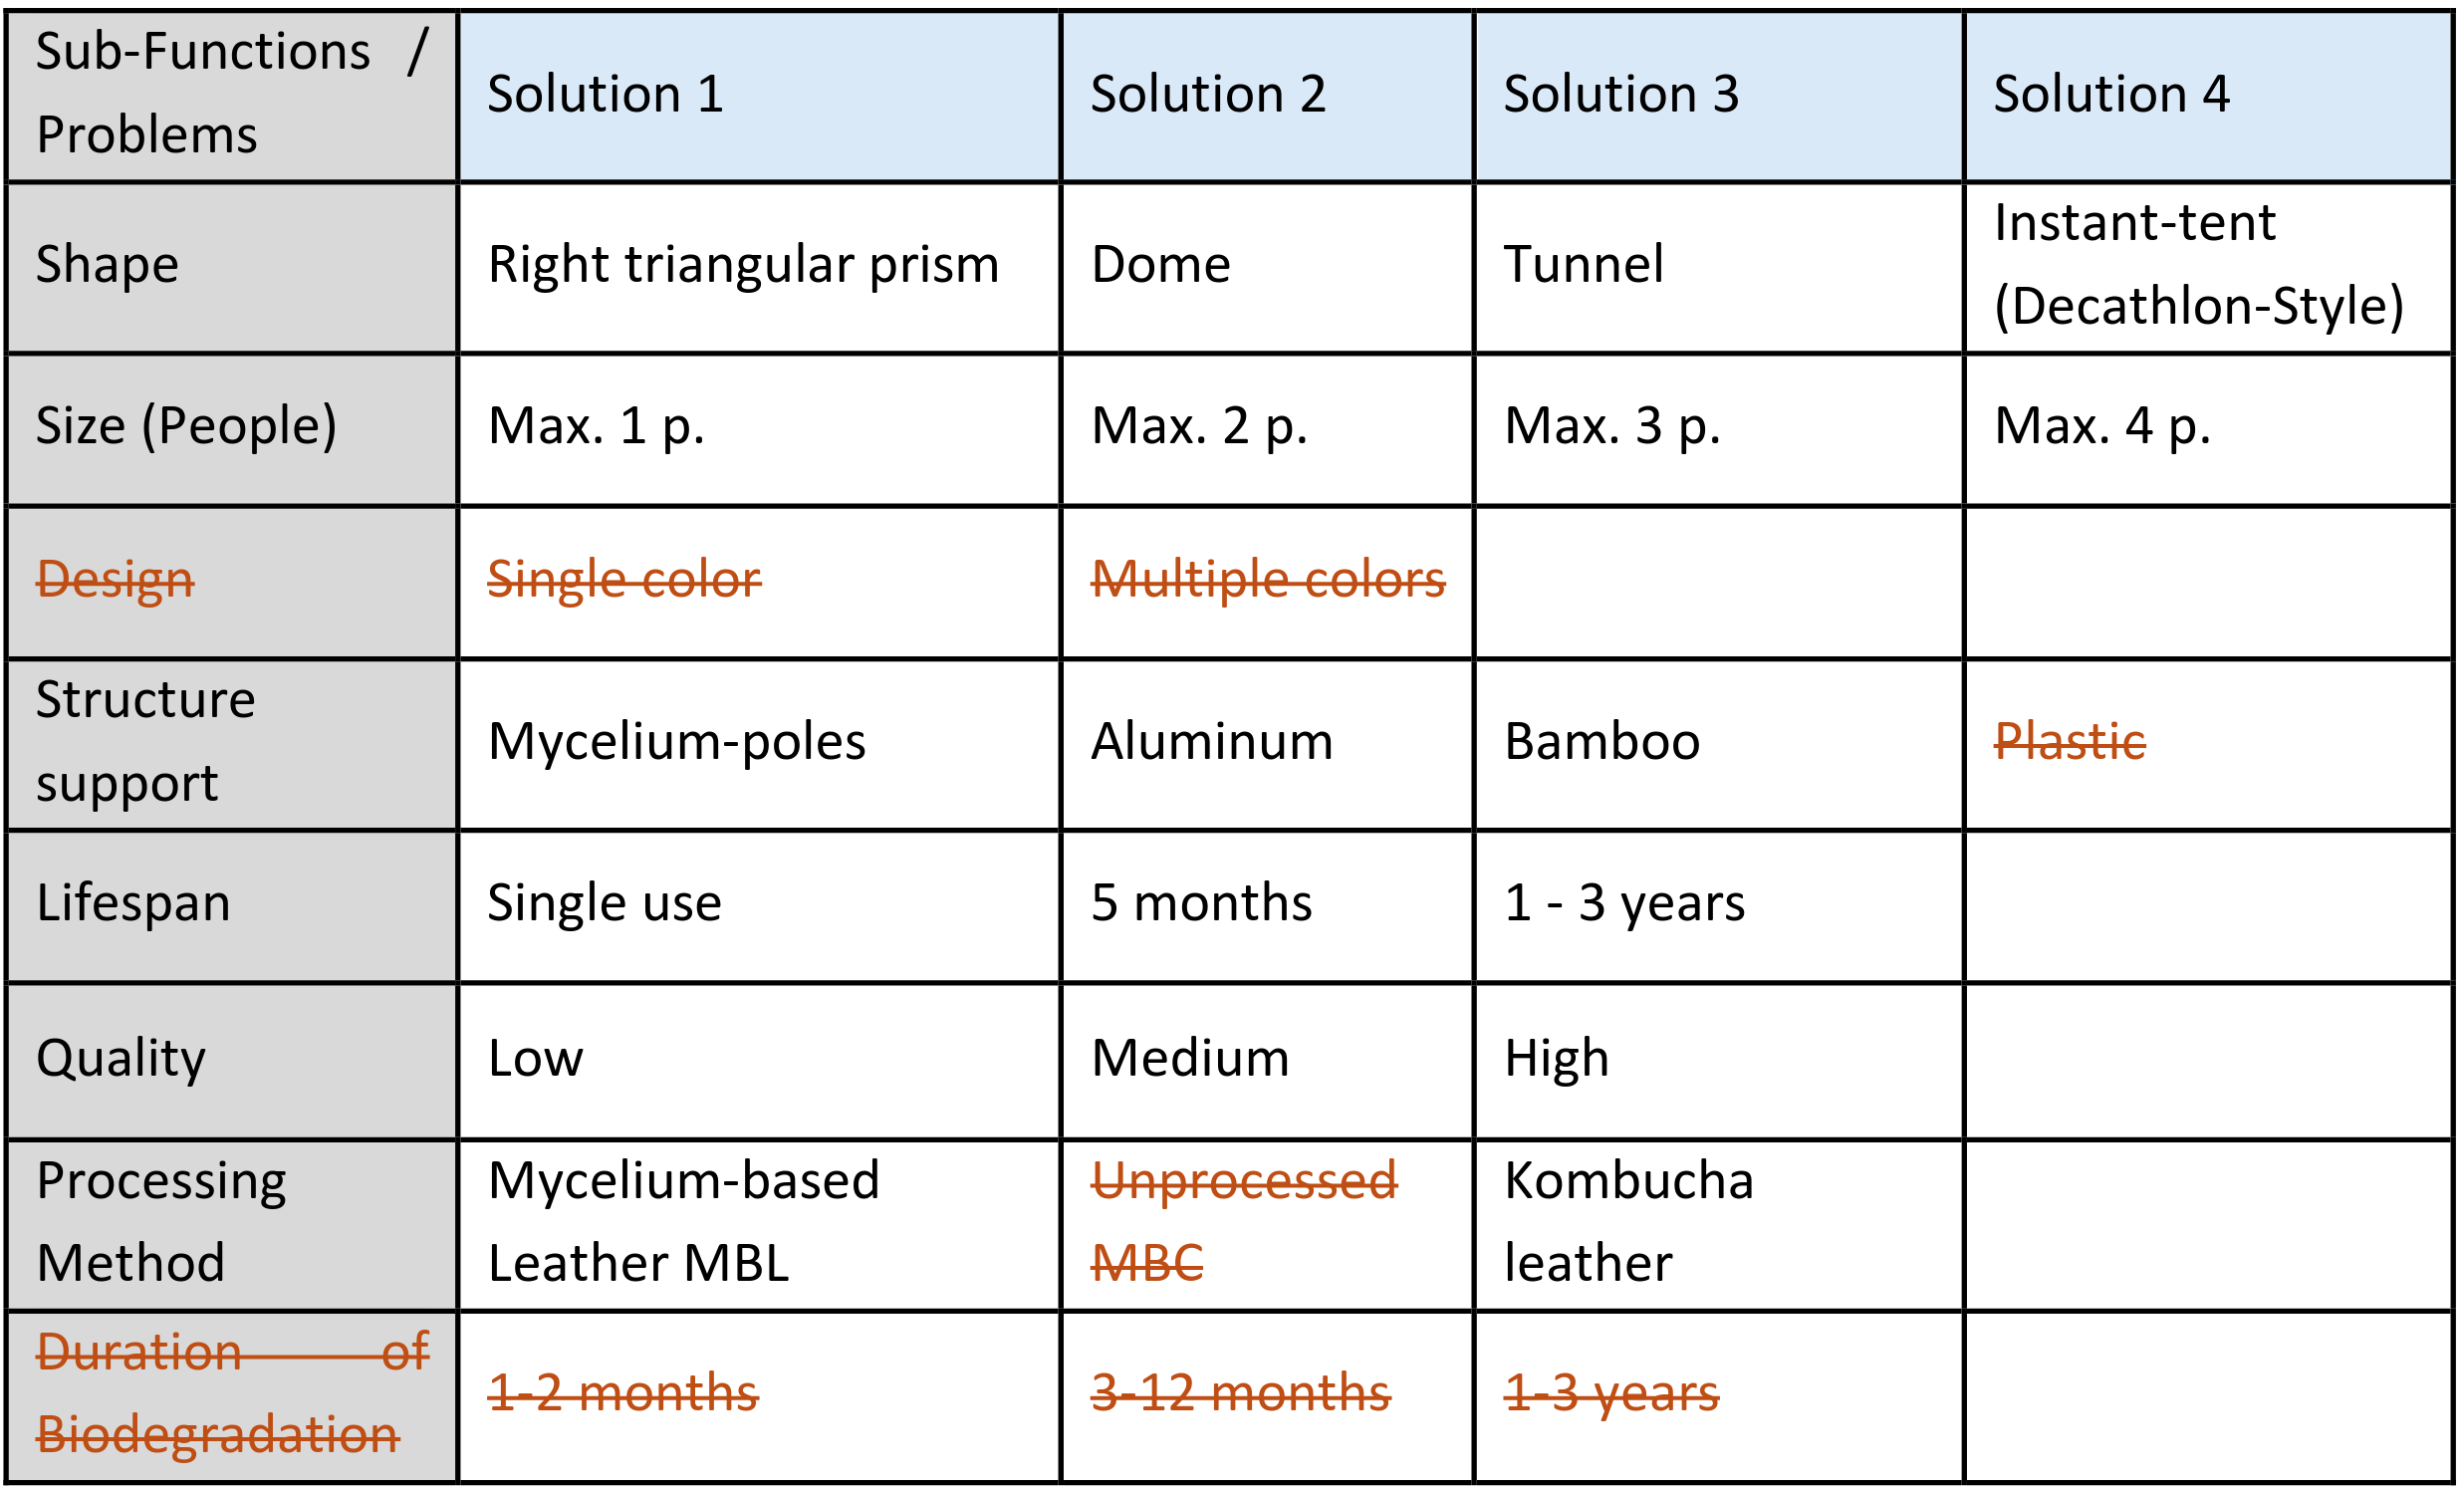
\includegraphics[width=\textwidth]{media/slimmed_morph.png}
\end{table}

\newpage
\pagestyle{empty}
\begin{figure}[ht!]
    \centering
    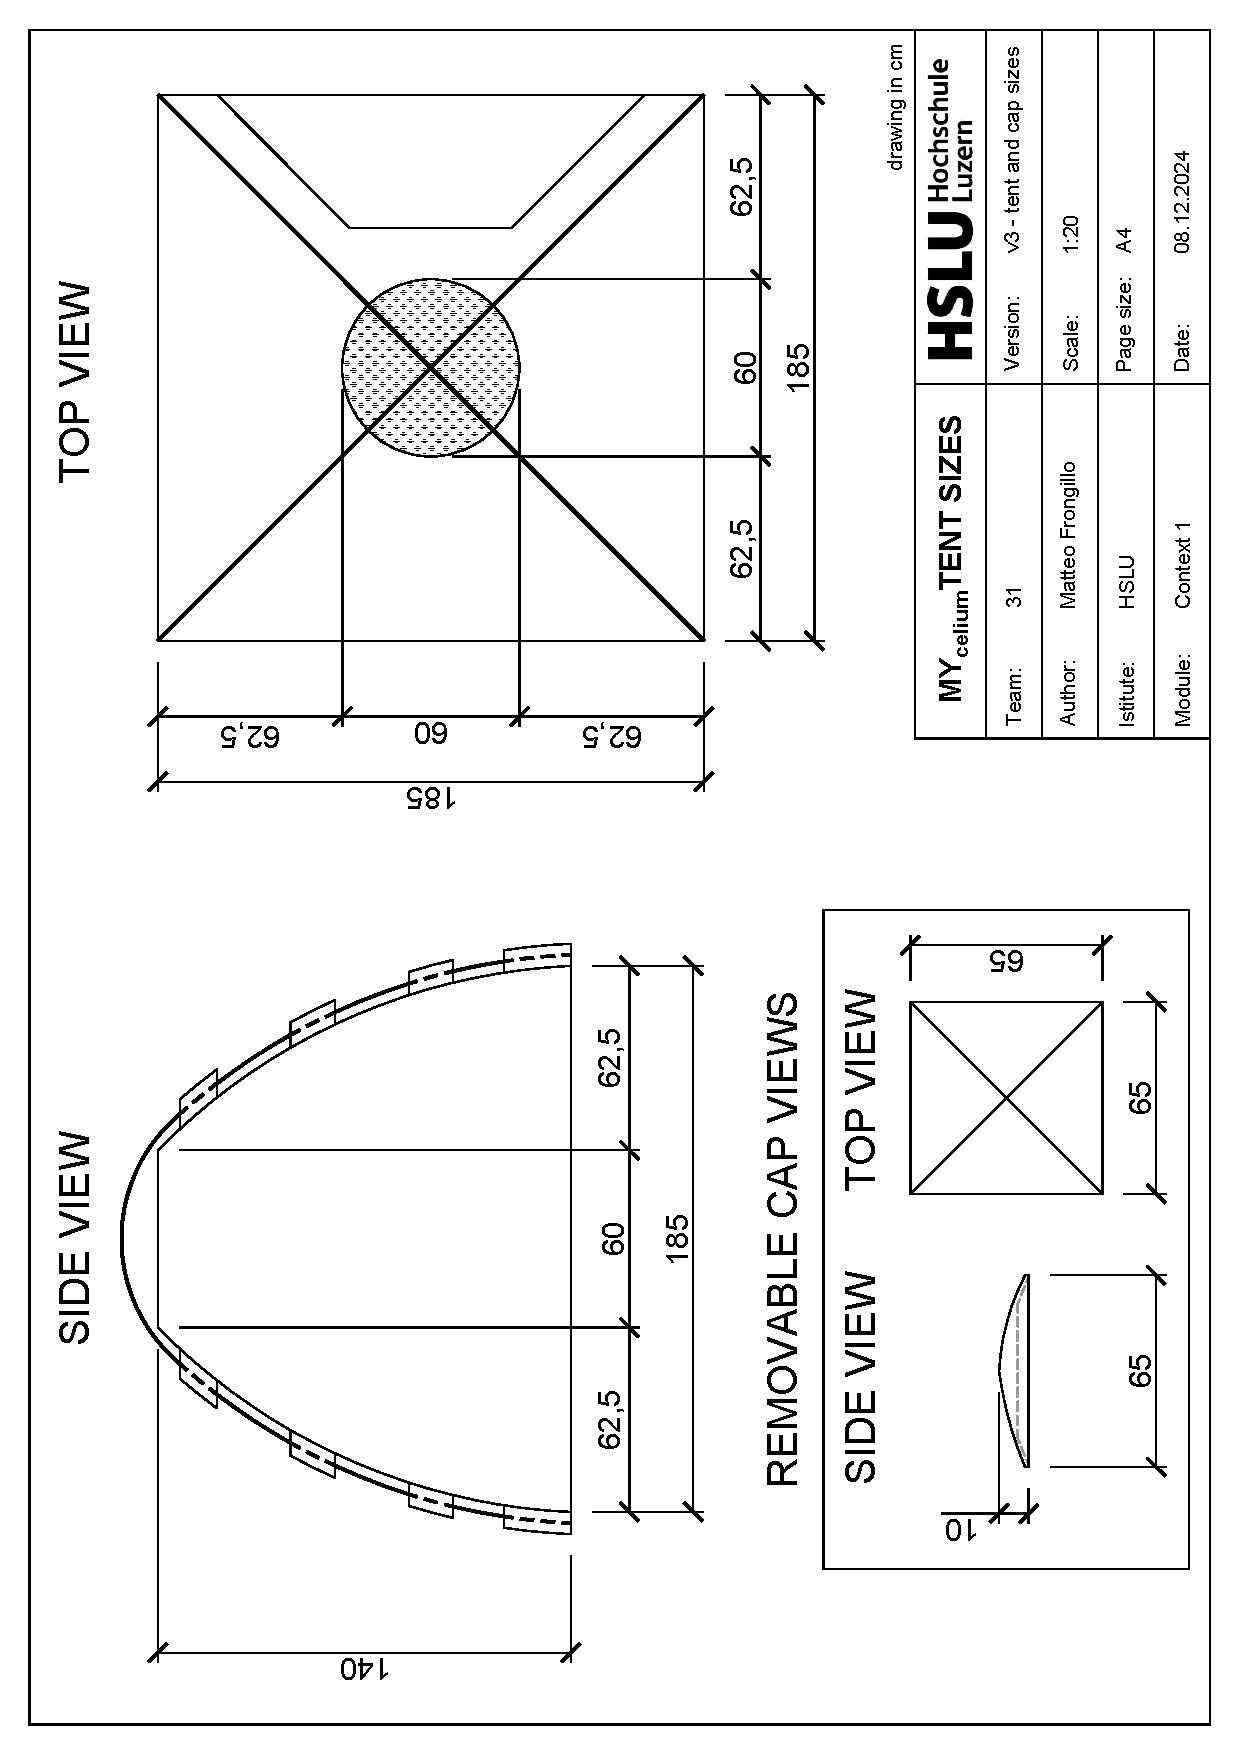
\includepdf[pages=1]{media/tent-size.pdf}
    \phantomcaption
    \label{pdf:tent-size}
\end{figure}
\addtocounter{figure}{+0}
\addcontentsline{lof}{figure}{\protect\numberline{\thefigure}Appendix: Tent size}

\newpage
\begin{figure}[ht!]
    \centering
    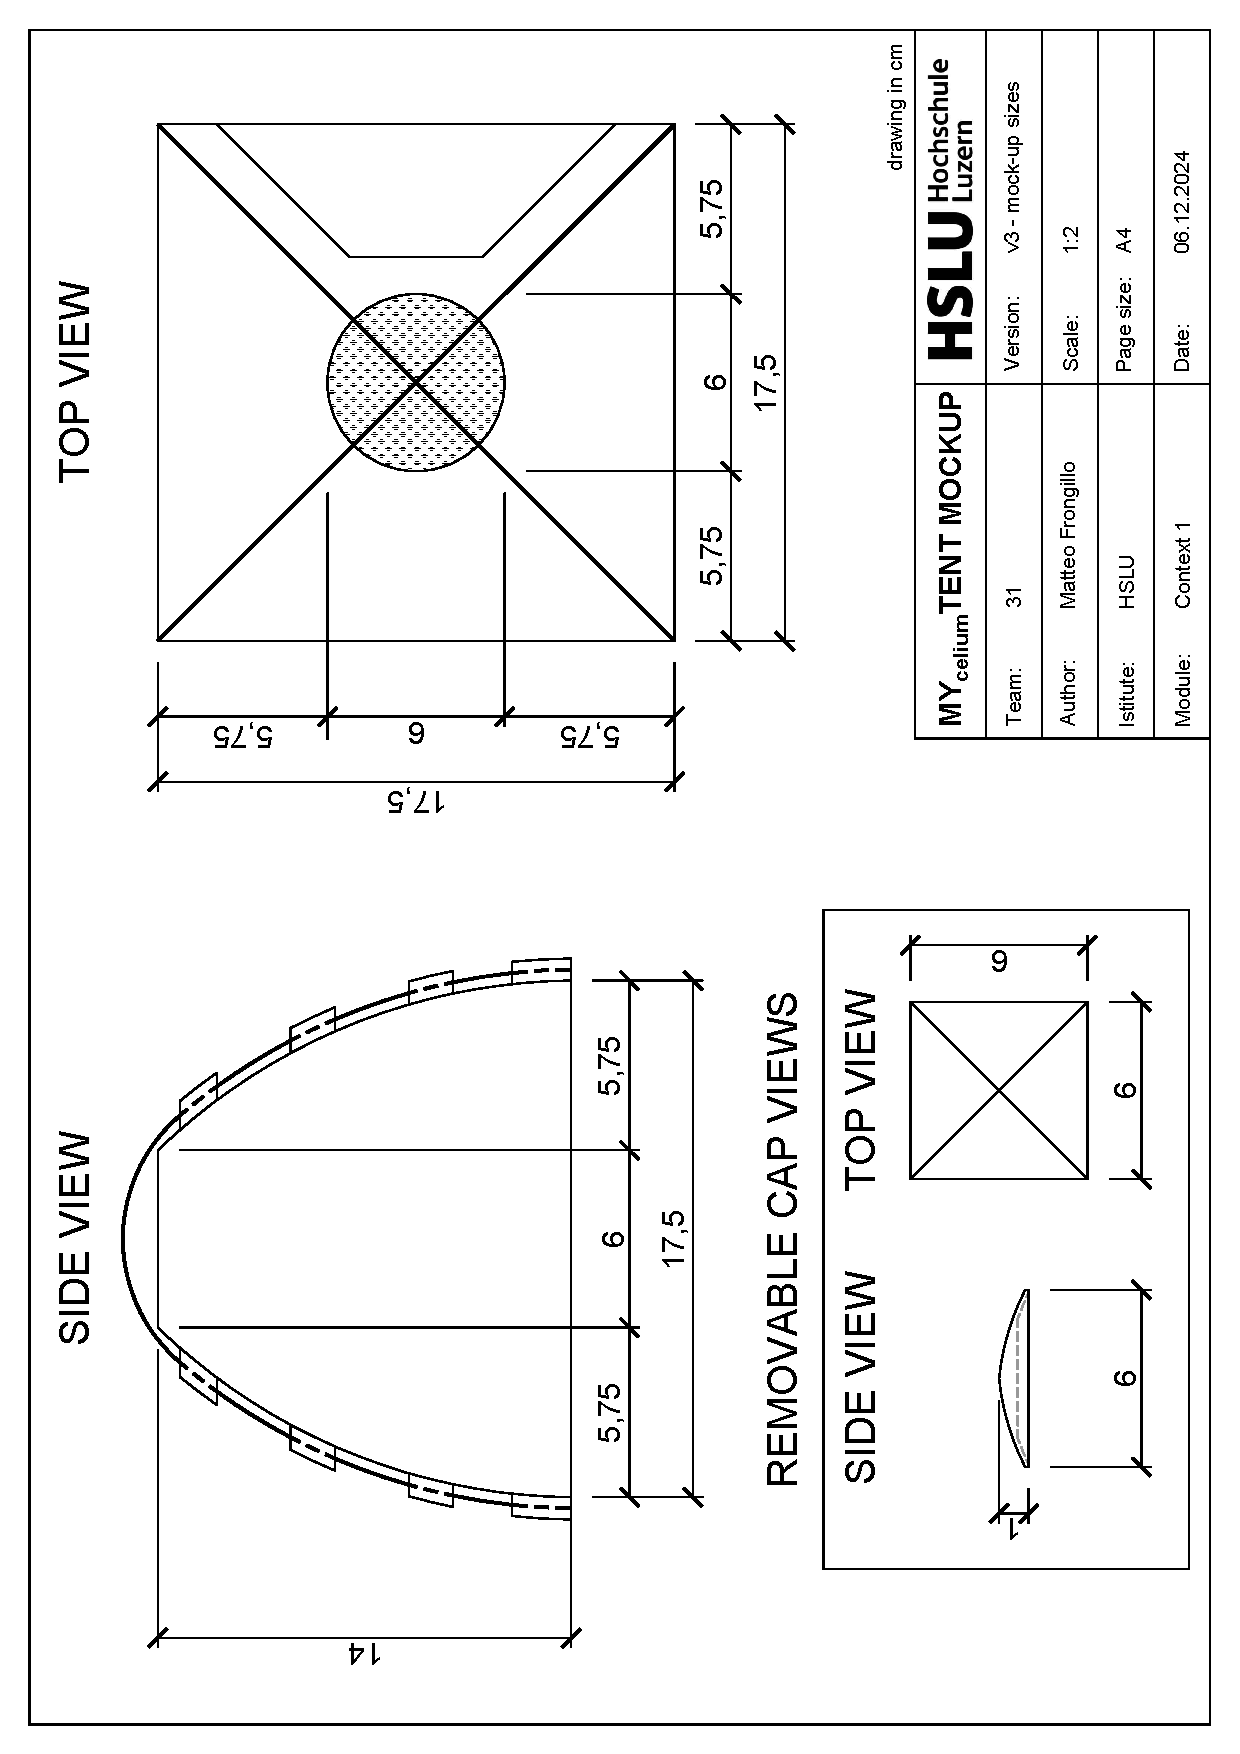
\includepdf[pages=1]{media/mockup-size.pdf}
    \phantomcaption
    \label{pdf:mockup-size}
\end{figure}
\addtocounter{figure}{+0}
\addcontentsline{lof}{figure}{\protect\numberline{\thefigure}Appendix: Mock-up size}

\end{document}

